\chapter{Implementation}
\label{chapter:implementation}

\section{Software Stack and Development Environment}
\label{section:software_stack_dev_environment}

To guarantee strict reproducibility, deterministic compilation, and seamless cross-platform deployment across Linux (Ubuntu) and Windows 
operating systems, the simulation framework incorporates a highly automated toolchain. The integration of native compiled code and 
high-level Python scripts is orchestrated uniformly at configuration time, eliminating manual dependency resolution and the classic 
"works on my machine" anti-pattern.

\subsection{Multi-Platform Build Automation and Toolchain}

The compilation pipeline relies on modern \texttt{CMake} (minimum version \texttt{4.1.1}) paired with \\ 
\texttt{CMakePresets.json} (version 9 schema) to standardize build configurations across varying host environments. 

\begin{itemize}
    \item \textbf{Compiler Specifications}: On Linux infrastructures, the toolchain enforces the GNU Compiler Collection 
    (\texttt{GCC/G++ 12}), while on Windows platforms, it targets the Microsoft Visual C++ (\texttt{MSVC 2026}) compiler. The codebase 
    strictly adheres to the \texttt{C++20} standard, utilizing compile-time concepts, parametric type resolution (via \texttt{std::variant} 
    visitors), and standard file system abstractions.

    \item \textbf{System Bootstrap and Build Backends}: On Linux environments, a low-level shell infrastructure script 
    (\texttt{install-deps.sh}) automates the ingestion of standard build prerequisites. It provisions the \texttt{build-essential} 
    metapackage alongside the \texttt{Ninja-build} daemon, which acts as the primary underlying meta-build generator to parallelize 
    translation units. Furthermore, it conditionally triggers graphical development dependencies (such as \texttt{libxinerama-dev}, \\
    \texttt{libxcursor-dev}, \texttt{xorg-dev}, and \texttt{libglu1-mesa-dev}) depending on whether a headless \\ \texttt{--server} execution 
    or a \texttt{--desktop} environment with GUI support is selected.
\end{itemize}

\subsection{Native C++ Dependency Management via vcpkg}

Native third-party libraries are fetched and compiled using Microsoft's \texttt{vcpkg} package manager executing in \textbf{Manifest Mode}. 

A defining feature for scientific validity is the declaration of a rigid \texttt{"builtin-baseline"}, explicitly locked to the Git commit hash:
\begin{center}
    \texttt{66c037dc7fca549e5803087b9487edfe3aca0a1}
\end{center}
This immutable anchor freezes the versioning matrix of every single compiled component down to its exact source tree revision, guaranteeing 
that any future compilation on arbitrary machines yields mathematically identical binary results. 

The dependency tree is segmented through modular manifest features, minimizing binary bloat by only activating required compilation targets:
\begin{enumerate}
    \item \textbf{Core Logging and Diagnostics}: Managed via \texttt{fmt} and \texttt{spdlog} (with integrated \texttt{fmt} support), 
    providing zero-allocation asynchronous string formatting.

    \item \textbf{Input and Boundary Ingestion}: Utilizing \texttt{nlohmann-json} for parsing geo-computational manifests and structural 
    metadata.

    \item \textbf{Output, Geospatial, and Network Infrastructure}: Powered by \texttt{opencv4} (configured with explicit \texttt{png} and 
    \texttt{jpeg} hardware compression codecs), \texttt{paho-mqttpp3} for asynchronous network transport synchronization, and 
    \texttt{geographiclib} alongside \texttt{magic-enum} to govern coordinate transformations and strongly-typed matrix boundaries.

    \item \textbf{Graphical User Interface}: Built upon the \texttt{imgui} framework (leveraging multi-backend bindings for \texttt{GLFW3} 
    and \texttt{OpenGL3}) and coupled with \texttt{portable-file-dialogs} for standard native OS dialogues.

    \item \textbf{Validation Layer}: Uses Google Test (\texttt{gtest}) for unit verification and behavioral testing.
\end{enumerate}

\subsection{Python Subsystems for Data Engineering and Deep Learning}

The simulation core does not operate as an isolated binary; it interacts with two specialized Python pipelines executing complementary 
stages of the digital twin lifecycles.

\subsubsection{Geospatial Pre-processing and Data Ingestion Pipeline}

Located within the \texttt{python/data\_pipeline} context, this subsystem is responsible for automated web-scraping, remote sensing API 
extraction, pluvial data gathering, and GIS structural alignment. It normalizes unstructured environmental parameters into 
tensor-compatible matrix files via a highly specific spatial stack:

\begin{itemize}
    \item \textbf{Geospatial Raster and Vector Operations}: \texttt{rasterio} and \texttt{fiona} provide low-level bindings to the 
    Geospatial Data Abstraction Library (GDAL), managing the read/write workflows of Digital Elevation Models (DEMs). Spatial 
    intersections, topological geometries, and coordinate reference system (CRS) transformations are resolved via \texttt{shapely} and 
    \texttt{pyproj}.

    \item \textbf{Mathematical and Stochastic Analysis}: \texttt{numpy} governs raw multi-dimensional matrix operations. Advanced 
    algorithmic spatial blending, watershed masking, and geo-statistical field configurations are achieved using \texttt{scikit-image} 
    and \texttt{gstools} (Random Field Generation).

    \item \textbf{Ingestion, Document Mining, and Visualization}: Web telemetry is harvested via \texttt{requests}, while official 
    hydrologic diagnostic reports distributed as tabular PDFs are scraped via \\ \texttt{pdfplumber}. Logging and diagnostic feedback are 
    decoupled through \texttt{loguru}, and configuration structures are mapped through \texttt{pyyaml}. Frame inspection is handled by 
    \texttt{matplotlib}.
\end{itemize}

\subsubsection{Neural Model Training and Parity Conversion Pipeline}

Located within the \texttt{python/models} context, this subsystem oversees the design, optimization, and structural translation of the 
Neural Operators that serve as the accelerated physical state solver.

\begin{itemize}
    \item \textbf{Tensor Computing Base}: Powered by \texttt{tensorflow==2.19.0}. This version provides absolute stability across both 
    industrial Linux containers and native Windows setups.

    \item \textbf{ABI and Memory Realignment Safeguard}: To guarantee cross-language pointer safety and avoid catastrophic memory 
    misalignment when binding tensors between Python environments and C++ buffers, the stack enforces \texttt{numpy<2.0}. This 
    restriction prevents the breaking changes introduced by the NumPy 2.0 ABI layout from corrupting raw memory mapping sequences.

    \item \textbf{Graph Compilation and Execution Parity}: The deep learning model is compiled into standard inference graphs via 
    \texttt{tf2onnx>=1.16.1}, setting specific Operator Set (Opset) directives. To ensure total behavioral parity and mathematical 
    convergence between the design environment and the C++ production execution, the local environment enforces 
    \texttt{onnxruntime==1.23.2}, matching precisely with the underlying runtime version ingested by \texttt{vcpkg} into the native 
    simulator application.
\end{itemize}

\subsection{Automated Virtual Environment Bootstrapping via CMake}

Rather than requiring manual system environment setups, the interaction between native builds and python subsystems is bridged by a 
custom automated pipeline defined in \texttt{python.cmake}. 

During the CMake configuration step, the script triggers a strict workflow:

\begin{enumerate}
    \item \textbf{Interpreter Discovery}: It checks for a native \texttt{Python3} interpreter matching precisely version \texttt{3.10} 
    or higher.

    \item \textbf{Isolated Environment Generation}: It dynamically detects the host operating system platform and spawns independent 
    virtual environments.

    \item \textbf{Dependency Enforcement}: It reads the respective local \texttt{requirements.txt} scripts, quietly executes an internal 
    system upgrade of \texttt{pip} to guarantee layer compatibility, and forces automated dependency installations inside the isolated 
    virtual environments without root or global scope contamination.

    \item \textbf{Path Injection Strategy}: To facilitate instant importing of internal cross-subsystem tools without relying on dangerous 
    dynamic environment overrides at runtime, the script automatically generates localized custom path configurations (\texttt{.pth} files) 
    and drops them directly into the target environment's \texttt{site-packages} directory. This guarantees zero-overhead tool discovery 
    across the software stack.
\end{enumerate}


\section{Core Engine and Multi-Physics Parallelization}

The computational efficiency of the $m:n-CA^k$ model relies on a hybrid execution strategy. The local transition rules and multi-physics 
equations are vectorized into a static data-flow graph using TensorFlow, which is subsequently compiled into an ONNX bytecode format. The 
runtime execution engine, implemented in native C++, wraps this graph and utilizes OpenMP to achieve multi-threaded, tile-based 
parallelization across CPU cores.

\subsection{Tensorized Transition Rules via TensorFlow/SIMD}

Traditional Cellular Automata implementations utilize nested loops to iterate over the spatial dimensions ($X \times Y$), checking the 
neighborhood state for each cell individually. This approach induces massive pointer-indirection and severely limits Single Instruction, 
Multiple Data (SIMD) hardware vectorization. 

To overcome this limitation, this simulator discards spatial loops entirely during the physics update phase. The transition rules are 
formulated as \textbf{tensorized stencil operations}. The spatial grid is treated as a contiguous multi-dimensional array, and neighborhood 
lookups are executed via vectorized tensor slicing and shifts. 

For the Moore neighborhood ($k=8$), the engine generates 8 distinct spatial slices from a padded representation of the global state tensors. 
For example, the total volumetric inflow ($\sum \Delta V_{in}$) for all celdas is computed simultaneously by shifting and adding the 
directional outflow tensors ($V_{out}$) using native array offsets:

\begin{lstlisting}[language=Python, caption=Tensorized Stencil for Inflow Accumulation]
# Vectorized accumulation of inflows from the 8 Moore neighbors
total_inflow = (
    outflow_padded[0, :, 2:,   1:-1] + # North
    outflow_padded[1, :, 0:-2, 1:-1] + # South
    outflow_padded[2, :, 1:-1, 0:-2] + # East
    outflow_padded[3, :, 1:-1, 2:]   + # West
    outflow_padded[4, :, 2:,   0:-2] + # North-East
    outflow_padded[5, :, 2:,   2:]   + # North-West
    outflow_padded[6, :, 0:-2, 0:-2] + # South-East
    outflow_padded[7, :, 0:-2, 2:]     # South-West
)
\end{lstlisting}

By transforming spatial iterations into element-wise matrix arithmetic, the underlying execution graph leverages low-level compiler 
optimizations such as loop unrolling, cache alignment, and hardware-level SIMD instructions (e.g., AVX-512). This allows millions of cells 
to update their hydraulic potential concurrently.

\subsection{Hydraulic Regime Switching in Code}

Evaluating multi-physics regimes (turbulent vs. laminar) within a localized cellular space typically introduces conditional branching 
(`if-else` statements). In parallel computing, spatial branching triggers severe performance degradation due to \textbf{branch misprediction} 
and thread divergence, as adjacent cells might follow different physical equations.

To maintain a pure mathematical stream, the multi-physics core implements a \textbf{branchless selection strategy}. Both the Turbulent velocity 
($v_{turb}$) and the Viscous/Laminar velocity ($v_{lam}$) are computed across the entire tensor space simultaneously. The physical selection 
is resolved via an element-wise mathematical minimum operator:

$$v_{approx} = \min(v_{turb}, v_{lam})$$

In the execution graph, this is mapped directly to the `tf.minimum` operator. When compiled into machine code via ONNX Runtime, this 
translates to hardware-level conditional selection instructions (such as `vminps` in x86 architectures). This completely bypasses the CPU's 
branch prediction unit, ensuring that the execution pipeline remains fully saturated regardless of whether a cell represents a turbulent 
mountain stream or a highly viscous mudflow in an urban basin.

\subsection{Boundary Conditions: The Impermeable Wall Logic}

The handling of the grid limits is essential to maintain the physical integrity and mass conservation of the simulation. In this model, 
boundary conditions are implemented using an absolute Virtual Wall strategy through specialized tensor padding applied directly to the 
hydraulic potential.

\paragraph{A. Water Surface Elevation (WSE) Formulation}

Before evaluating spatial transitions and boundary interactions, the execution core couples the static terrain and dynamic fluid columns. 
For each cell, the total potential energy is defined by the Water Surface Elevation ($WSE$), algebraically computed as the sum of the 
Topobathymetry ($Z_{topo-bathy}$) and the current Water Depth ($WD$):

$$WSE_{i,j} = Z_{topo-bathy, i,j} + WD_{i,j}$$

\paragraph{B. Insurmountable Constant Tensor Padding}

To enforce a strict non-building, impermeable boundary condition (Zero-Flux Boundary) at the grid edges, the engine does not pad physical 
layers independently. Instead, a static spatial border is injected into the combined $WSE$ tensor utilizing a Constant Padding strategy 
with an insurmountable virtual height threshold ($\mathcal{H}_{wall} = 9999.0\text{ m}$):

$$\text{Padding}(WSE, \text{mode='CONSTANT'}, \text{constant\_values}=\mathcal{H}_{wall})$$

This formulation forces the transition logic to treat the exterior of the computational matrix as an infinitely high topographic ridge. 
Because the intra-layer propagation engine calculates flow velocities and multi-directional routing based on positive potential energy 
gradients ($S_k > 0$), any cell located at the absolute border of the study area will compute a heavily negative gradient toward the 
exterior:

$$S_{border} = \frac{WSE_{border\_cell} - \mathcal{H}_{wall}}{L_k} \ll 0$$

Adhering to the physical constraints of the model, gradients where $S_k \le 0$ are completely ignored. Consequently, water is mathematically 
prohibited from escaping the active matrix boundaries, successfully simulating a perfectly contained hydrologic environment. This absolute 
"Wall" logic is critical for modeling the urban sub-basins of the Valencia DANA scenario, preventing numerical mass loss at the bounds of 
the digital elevation models.

\subsection{Numerical Stability: Spatial and Temporal Volumetric Shields}

To guarantee strict mass conservation and suppress numerical oscillations (such as hydraulic gradient inversions or checkerboard 
instabilities), the execution graph introduces a dual-stage volumetric limiting mechanism. Traditional hydrodynamic models rely on 
strict adaptive time-stepping (CFL criteria) which forces global synchronization. In contrast, this tensorized core applies localized, 
element-wise \textbf{Spatial and Temporal Shields} directly onto the multi-directional outflow vectors.

\paragraph{A. The Spatial Shield (Level Equalization)}

When a cell updates its state, an unconstrained transition rule could route an excessive volume of water toward a lower neighbor, dropping 
the source cell's Water Surface Elevation ($WSE$) below that of its destination. This induces a non-physical hydraulic gradient inversion in 
the next time-step, causing severe numerical waves. 

To prevent this, the \textit{Spatial Shield} limits the maximum allowable volumetric drop. A cell is prohibited from lowering its water 
level beyond half of the maximum elevation difference with its lowest neighbor within the Moore neighborhood:

$$\Delta V_{\text{spatial}} = \frac{\max(\Delta WSE) \cdot \Delta x^2}{2}$$

Where $\max(\Delta WSE)$ represents the maximum positive potential energy gradient calculated across the active neighborhood slices, and 
$\Delta x^2$ denotes the cell area ($A_{\text{cell}}$).

\paragraph{B. The Temporal Shield (Volumetric CFL Condition)}

Concurrently, the model must ensure that the total combined outflow from a single cell does not exceed its actual physical fluid mass in a 
single step, which would result in negative water depths. The total available volume ($V_{\text{avail}}$) is thus bounded by both the 
physical water column volume ($V_{\text{cell}} = WD \cdot \Delta x^2$) and the spatial restriction:

$$V_{\text{avail}} = \min(V_{\text{cell}}, \Delta V_{\text{spatial}})$$

\paragraph{C. Branchless Proportional Scaling}

If the sum of all theoretical directional outflows ($\sum \Delta V_{\text{theor}, k}$) computed by the physics regimes exceeds 
$V_{\text{avail}}$, the outflows must be scaled down proportionally to preserve the physical multi-directional routing ratios. 

To maintain the \textbf{branchless execution strategy} detailed in Section 4.2 and avoid CPU thread divergence, this optimization is 
achieved via an element-wise scale factor ($\alpha$). The reduction factor is computed utilizing a safe, non-zero division operator:

$$\alpha = \frac{\min\left(\sum \Delta V_{\text{theor}, k}, V_{\text{avail}}\right)}{\sum \Delta V_{\text{theor}, k}}$$

\begin{lstlisting}[language=Python, caption=Tensorized Volumetric Shields and Safe Scaling]
# 4. SPATIAL SHIELD: Max allowable volume drop to prevent inversion
max_delta_wse = tf.reduce_max(delta_wse_positive, axis=0)
delta_V_spatial = (max_delta_wse * cell_area) / 2.0

# 5. TEMPORAL SHIELD: Volumetric constraint based on physical mass
V_cell = water_depth * cell_area
V_avail = tf.minimum(V_cell, delta_V_spatial)

# Total theoretical outflow attempt across all k-directions
total_outflow_attempt = tf.reduce_sum(delta_V_theor_k, axis=0)

# Branchless proportional scaling factor (alpha)
alpha = tf.math.divide_no_nan(
    tf.minimum(total_outflow_attempt, V_avail), 
    total_outflow_attempt
)

# Safe and volumetrically continuous directional outflows
delta_V_out_k = delta_V_theor_k * alpha
\end{lstlisting}

By mapping this algebraic correction directly into `tf.math.divide\_no\_nan` and `tf.minimum`, the compiler translates the safety constraints 
into hardware-level SIMD operations. This ensures complete volumetric continuity and numerical stability across highly irregular 
topographies (such as flash floods in urban catchments) without breaking the saturation of the execution pipeline.

\subsection{Hybrid Thread-Level Parallelism via C++ and OpenMP}

While the core physics transitions are encapsulated within the tensor graph, the macro-management of the simulation space is orchestrated 
by a multi-threaded C++ wrapper (\texttt{OnnxStateUpdater}). 

To optimize performance on large river basins, the C++ engine implements an active-tile scheduling mechanism. The total grid space is 
segmented into localized sub-blocks. Before launching the tensor graph inference, the engine queries the Water Movement State layer 
($E_5$) to filter out entirely static or dry tiles, creating a localized dynamic bounding box.

The management of these active tiles, alongside the post-processing classification of the Flood Risk layer ($E_6$), is parallelized across 
multiple CPU cores using OpenMP directives:

\begin{lstlisting}[language=C++, caption=OpenMP Parallelization for Risk Classification and State Management]
#pragma omp parallel for schedule(dynamic)
for (int64_t i = 0; i < total_cells; ++i) {
    // Thread-safe extraction of localized cell data
    float current_depth = water_depth_ptr[i];
    
    // Real-time heuristic hazard mapping (E6 Evolution)
    flood_risk_ptr[i] = ClassifyRisk(current_depth);
    
    // Dynamic update of the active shielding layer (E5 Evolution)
    if (current_depth > dry_tolerance) {
        wms_ptr[i] = static_cast<int8_t>(WaterMovementState::kDynamicState);
    } else {
        wms_ptr[i] = static_cast<int8_t>(WaterMovementState::kStaticState);
    }
}
\end{lstlisting}

By combining the \textbf{Data-Level Parallelism (DLP)} of the TensorFlow-ONNX graph with the \textbf{Thread-Level Parallelism (TLP)} of OpenMP, the 
simulation engine establishes a highly scalable framework capable of handling high-resolution GIS datasets under real-time operational 
constraints.


\section{Hexagonal Architecture Layout}

\subsection{Directory Topology and Project Modules}

To enforce the conceptual boundaries established by the Hexagonal Architecture \ref{sec:hexagonal-methodology}, the physical source 
code is strictly partitioned into isolated modules. The directory layout separates the mathematically pure simulation domain from 
infrastructure-dependent adapters, data ingestion services, and presentation layers. The structural topology of the project is 
organized as follows:

\begin{figure}[htbp]
    \centering
    \footnotesize
    \begin{forest}
      for tree={
        folder,   
        font=\ttfamily,
        grow'=0,
      }
    [app
        [adapters
            [input]
            [output]
            [state\_updater]
        ]
        [config]
        [core
            [grid
                [layers]
                [scalars]
            ]
            [ports]
            [snapshot]
        ]
        [io
            [readers]
            [writers]
        ]
    ]
    \end{forest}
    \caption{Project directory topology reflecting the Hexagonal Architecture modules.}
    \label{fig:directory_topology}
\end{figure}

The architectural responsibilities of these primary directories are detailed below:

\begin{itemize}
    \item \textbf{The Simulation Core (\texttt{app/core}):} This module represents the absolute ``Inside'' of the hexagon, containing 
    zero external dependencies. 

    \begin{itemize}
        \item \texttt{grid/}: Manages the multi-layered spatial data structures. The \texttt{layers/} submodule stores the multi-channel 
        grid tensors, while \texttt{scalars/} handles global variables such as critical time-steps ($\Delta t$) or fluid density.

        \item \texttt{ports/}: Defines the pure abstract interfaces (both driving and driven) that the core exposes to interact with 
        data sources and sinks.

        \item \texttt{snapshot/}: Manages saved instances of the simulation's world state. This allows the computational engine to 
        continue executing subsequent time-steps uninterrupted while the defined output ports concurrently read the captured states, 
        preventing resource locking and data corruption.
    \end{itemize}

    \item \textbf{Infrastructure Adapters (\texttt{app/adapters}):} This directory bridges the core interfaces with real-world 
    technical implementations. 

    \begin{itemize}
        \item \texttt{input/}: Implements the driving adapters responsible for reading external data sources and transforming them 
        into the specific multi-channel tensor formatting required by the internal simulation grid layout.

        \item \texttt{output/}: Houses the driven adapters tasked with processing the captured snapshots of the world state. This 
        module handles the translation of these snapshots into multiple concrete formats, including system checkpoints for simulation 
        recovery, localized spatial images for physical storage, and asynchronous MQTT payloads for real-time remote telemetry.

        \item \texttt{state\_updater/}: Contains the execution workers responsible for driving the simulation forward through discrete 
        temporal steps. It orchestrates the cellular automata execution, computing the transition rules to evolve the entire system 
        state from time-step $t$ to $t+1$.
    \end{itemize}

    \item \textbf{Data Ingestion and Pipelines (\texttt{app/io}):} A dedicated subsystem for heavy file manipulation and GIS translation. 
    The \texttt{readers/} and \texttt{writers/} submodules are decoupled into \texttt{static} (e.g., digital elevation models, soil types) 
    and \texttt{dynamic} (e.g., temporal rainfall series) streams, ensuring optimal memory-mapped file access.
\end{itemize}


\subsection{Implementation of Ports / Abstract Contracts}
\label{subsec:implementation_ports}

In C++, abstract ports are implemented as pure abstract classes containing pure virtual functions ($=0$) and virtual destructors. 
This ensures compile-time decoupling, forcing infrastructure adapters to strictly adhere to the signatures required by the simulation 
core. Based on the project requirements, three primary abstract ports were developed to manage data ingestion, state mutation, and 
result serialization.

\subsubsection{Data Ingestion Contract: InputPort}

The \texttt{InputPort} interface establishes how the core requests environmental and geographical datasets without bound to specific 
file systems or database APIs. 

\begin{itemize}
    \item \textbf{Abstract Factory Pattern}: The port utilizes an abstract factory method, \texttt{GenerateReader()}, which returns 
    a \texttt{std::unique\_ptr<io::readers::Reader>}. This enforcement ensures that the core safely manages the lifecycle of polymorphic 
    reader instances via smart pointers, completely ignoring whether the underlying driver is reading a local binary file or parsing 
    a network stream.
    
    \item \textbf{Metadata Queries}: Methods such as \texttt{IsStaticLayer()} and \texttt{GetDatasetName()} allow the core to query 
    properties of the incoming dataset to dynamically allocate the multi-channel grid layers before data stream compilation.
\end{itemize}

\subsubsection{Asynchronous Execution Contract: OutputPort}

The \texttt{OutputPort} interface is fundamentally designed around performance isolation to prevent heavy I/O operations (such as 
writing physical files to disk or streaming chunks over the network) from bottlenecking the main simulation loop.

\begin{itemize}
    \item \textbf{Thread Context Isolation}: As declared in the contract, implementations of this port are intended to run inside 
    their own independent thread contexts via the \texttt{Run()} method.
    
    \item \textbf{Thread-Safe Data Consumers}: The \texttt{Run()} method accepts a reference to a thread-safe 
    \texttt{snapshot::SnapshotManager}. This mechanism allows the adapter implementation to continuously pull available simulation 
    states from a concurrent queue in a non-blocking fashion until a shutdown signal is dispatched.
    
    \item \textbf{Initialization Lifecycle}: The interface enforces a \texttt{SetInitConfig()} method, ensuring that any output 
    consumer receives structural metadata, spatial dimensions, and localized hazard classification thresholds (\texttt{FloodRiskLevel}) 
    prior to thread execution.
\end{itemize}

\subsubsection{Numerical Solver Contract: StateUpdaterPort}

The \texttt{StateUpdaterPort} serves as the boundary interface for the explicit physical solver execution. It encapsulates the core 
analytical parameters while remaining generic enough to support multiple computational backends (e.g., CPU, GPU, or cellular automata 
matrix engines).

\begin{itemize}
    \item \textbf{State Optimization Tracking}: The port introduces an internal optimization tracking mechanism via the 
    \texttt{WaterMovementState} enumeration. It classifies grid nodes into \texttt{kStaticState} (dry or stationary nodes where fluxes 
    are bypassed) and \texttt{kDynamicState} (kinetic cells with active flux propagation). This contract forces any concrete solver 
    implementation to exploit spatial sparsity to optimize computational throughput.
    
    \item \textbf{Encapsulated Forcing Parameters}: The interface manages immutable configuration blocks required for temporal 
    transitions, such as pluvial forcing toggles (\texttt{enable\_rainfall\_}), structural safety limits (\texttt{dry\_tolerance\_}), 
    and pre-defined risk vector layers used to map water depths into hazard severities during the $t \rightarrow t+1$ transition.
\end{itemize}


\subsection{Implementation of Infrastructure Adapters}

\subsubsection{Implementation of Driving Adapters: Input Infrastructure}

Driving adapters (or primary adapters) are positioned at the boundary of the infrastructure layer, tasked with capturing external 
data and delivering it to the Core through the abstract contracts described in Section~\ref{subsec:implementation_ports}. At the 
current development stage, the data ingestion pipeline relies on a specialized file-system adapter, \texttt{FileInput}, which 
materializes the \texttt{InputPort} interface.

\paragraph{The FileInput Adapter Component}

The \texttt{FileInput} class, encapsulated within the \texttt{floodsim::app::adapters::input} namespace, acts as a high-level file 
manager that maps physical workspace directories into structured logical layers. It manages configurations for both immutable 
geographic constraints (such as digital elevation models) and time-variant datasets (such as pluvial hydrographs).

\begin{itemize}
    \item \textbf{Filesystem Path Resolution}: The class constructor accepts a root \texttt{std::filesystem::path} alongside a 
    specific \texttt{dataset\_name} string. Upon initialization, it safely constructs a target environment path by utilizing modern 
    C++ operator overloading (\texttt{data\_path / dataset\_name}). This ensures cross-platform compatibility regarding directory 
    separation tokens (e.g., forward vs. backward slashes) without embedding hardcoded strings into the compiled binary.
    
    \item \textbf{Polymorphic Generation via Factory Delegation}: The core method \texttt{GenerateReader()} overrides the abstract 
    port contract to instantiate concrete file parsers dynamically. Rather than hardcoding specific file-parsing logic, 
    \texttt{FileInput} acts as a router that delegates instantiation to dedicated static and dynamic reader factories:

    \begin{itemize}
        \item If the requested layer is flagged as static (\texttt{is\_static == true}), it invokes the static factory: \\
        \texttt{io::readers::file::FileStaticReaderFactory::Create()}.
        \item If the layer holds time-variant arrays, it invokes the dynamic factory: \\
        \texttt{io::readers::file::FileDynamicReaderFactory::Create()}.
    \end{itemize}

    Both factories accept strongly-typed formatting enums (\texttt{FileStaticFormat} and \texttt{FileDynamicFormat}), binding the 
    abstract \texttt{std::unique\_ptr<io::readers::Reader>} return envelope to a concrete format parser (such as native IDRISI raster files).
    
    \item \textbf{Layer Property Introspection}: The adapter implements \texttt{IsStaticLayer()} by querying the underlying 
    \texttt{FileStaticReader} definition block. This allows the Core to query whether a named data source requires continuous 
    stream synchronization or single-step memory initialization before launching the simulation loop.
    
    \item \textbf{Cross-Cutting Observability}: To provide systemic diagnostic capabilities, the constructor triggers an explicit 
    logging call (\texttt{LOG\_INFO}) injecting the resolved workspace path string via \texttt{input\_path\_.string()}. This establishes 
    auditability, validating the correct initialization of boundary parameters prior to matrix allocation.
\end{itemize}

\subsubsection{Implementation of Driven Adapters: Output Infrastructure}
\label{subsec:output_adapters_implementation}

Driven adapters (or secondary adapters) are invoked by the Core to export calculation results, save state checkpoints, or stream live 
data to remote interfaces. To prevent slow disk write cycles or network latency from blocking the explicit numerical solver, these 
adapters implement the asynchronous thread execution model enforced by the \texttt{OutputPort} contract.

\paragraph{Polymorphic Lifetime Management: OutputFactory}

The instantiation of output adapters is decoupled from the main simulation initialization using a centralized factory. The 
\texttt{OutputFactory} class utilizes a modern compile-time functional pattern leveraging C++20 features:

\begin{itemize}
    \item \textbf{Type-Safe Variant Inversion}: The configuration of desired outputs is stored within a collection of \texttt{std::variant} 
    types. To resolve concrete types without resorting to expensive runtime type information (RTTI) or cascading \texttt{if-else} 
    statements, the factory utilizes the \texttt{std::visit} operator paired with a custom \texttt{Overloaded} pattern-matching structure:

\begin{lstlisting}[language=C++]
template <class... Ts> struct Overloaded : Ts... { using Ts::operator()...; };
template <class... Ts> Overloaded(Ts...) -> Overloaded<Ts...>;
\end{lstlisting}

    This pattern permits passing a unified block of anonymous lambda functions to parse configuration entries dynamically, returning a 
    vector of polymorphic smart pointers \\(\texttt{std::vector<std::unique\_ptr<core::ports::OutputPort>>}) bound to their respective 
    infrastructure drivers.
\end{itemize}

\paragraph{State Persistence and Recovery: CheckpointOutput}

The \texttt{CheckpointOutput} adapter targets physical storage to archive comprehensive simulation snapshots, ensuring fault tolerance 
and reproducibility.

\begin{itemize}
    \item \textbf{I/O Framework Delegation}: Upon instantiation, the class requests a concrete binary file writer from 
    \texttt{io::writers::file::FileStaticWriterFactory}. In the execution loop, the adapter safely unwraps incoming snapshots from 
    the concurrent queue, mapping multidimensional tensor slices (such as water depth arrays) directly onto storage.
    
    \item \textbf{Cross-Platform Filework Protection}: To prevent OS-specific path parsing conflicts, the method 
    \texttt{SaveSnapshotAsCheckpoint()} captures the simulation ISO-8601 timestamp string and sanitizes file token hierarchies, 
    replacing illegal naming parameters (such as colons \texttt{':'} on Windows platforms) with standard delimiters (\texttt{'-'}) 
    prior to creating structured directory trees with \texttt{std::filesystem::create\_directories()}.
\end{itemize}

\paragraph{Asynchronous Real-Time Telemetry: MqttOutput}

For distributed network synchronization, the \texttt{MqttOutput} adapter implements a custom network protocol over an asynchronous MQTT 
broker client, optimizing wide-area telemetric transmission.

\begin{itemize}
    \item \textbf{Network Bandwidth Optimization (Chunking Mechanism)}: Transmitting raw high-resolution grid tensors over network 
    sockets would induce buffer overflows. To overcome this infrastructure limit, the adapter implements a specialized chunking mechanism 
    controlled by structured macro parameters (\texttt{kChunkSize = 40000} cells, \texttt{kBatchSize = 10}). Instead of broadcasting 
    the monolithic matrix, the adapter maps grid differential arrays (\texttt{core::snapshot::ChangeList}) and breaks them into 
    localized telemetry payloads.
    
    \item \textbf{Handshake and Stream Synchronization Lifecycle}: The message workflow adheres to a strict framing protocol:
    \begin{enumerate}
        \item A frame initialization notice (\texttt{FrameStart}) is pushed to the transmission topic.

        \item The adapter streams the serialized chunks in sequential batches. For every batch window, the thread enters a brief 
        control cycle, subscribing to a localized feedback channel (\texttt{ChunkAck}) to confirm remote consumption before 
        releasing subsequent packets.

        \item Once complete, it dispatches \texttt{FrameEnd} and a temporal synchronization payload (\texttt{FrameSync}) containing 
        the precise snapshot timestamp to coordinate remote rendering frameworks.
    \end{enumerate}
    
    \item \textbf{Interoperable Serialization Inversion}: Payloads are managed through an abstract \texttt{PayloadSerializer} strategy 
    interface, currently defaulting to a concrete \texttt{JsonSerializer} handler. This design isolates the data format from network 
    sockets, allowing future upgrades to binary serialization engines (e.g., Google Protocol Buffers or FlatBuffers) without mutating 
    the core network pipeline.
\end{itemize}

\paragraph{Visual Analytics Canvas: ImageOutput}

To satisfy immediate spatial understanding and emergency analysis, the \texttt{ImageOutput} adapter provides automated graphical 
asset rendering directly from spatial calculations.

\begin{itemize}
    \item \textbf{Matrix Fusion Framework}: This component integrates the OpenCV graphics engine (\texttt{cv::Mat}) to perform 
    multi-layer matrix arithmetic. It fetches raw float arrays representing the localized topography and bathymetry 
    (\texttt{topo\_bathy\_}) and overlays the calculation state. The system computes a weighted arithmetic blend to superimpose 
    dynamic water vectors on top of the terrain background:

\begin{lstlisting}[language=C++]
dst_ptr[c] = cv::Vec3b(
    static_cast<uchar>(w_col[0] * 0.85 + t_col[0] * 0.15),
    static_cast<uchar>(w_col[1] * 0.85 + t_col[1] * 0.15),
    static_cast<uchar>(w_col[2] * 0.85 + t_col[2] * 0.15)
);
\end{lstlisting}

    This pixel-level transformation applies an alpha-blending ratio ($85\%$ fluid weight vs. $15\%$ terrain base) providing clear 
    visual transparency.
    
    \item \textbf{Dynamic Canvas Expansion}: Rather than exporting an unadorned matrix raster, the class constructs an extended 
    graphical canvas by allocating extra pixel spaces via custom layout boundaries (\texttt{margin\_title} and \texttt{sidebar\_width}). 
    It delegates UI pipelines through a localized \texttt{DrawUI()} matrix utility to stamp dynamic elements, including active simulation 
    timestamps, spatial dimension matrices, and hazard risk banners (\texttt{FloodRiskLevel} color lookup definitions) before finalizing 
    PNG image compression.
\end{itemize}


\subsubsection{Implementation of Simulation Workers: State Updater Infrastructure}
\label{subsec:state_updater_implementation}

The state updater infrastructure represents the mathematical and computational core of the simulation's physical execution. In accordance 
with Hexagonal Architecture, this module materializes the \texttt{StateUpdaterPort} contract, translating the multi-channel spatial 
state of the domain from time-step $t$ to $t+1$. Rather than relying on traditional, slow numerical solvers, the architecture decouples 
physics through an inference pipeline powered by the ONNX Runtime C++ framework.

\paragraph{The Simulation Engine Factory: StateUpdaterFactory}

To support multiple computational backends and protect the Core from direct dependencies on foreign runtime APIs, instantiation is 
inside the \texttt{StateUpdaterFactory}. 

\begin{itemize}
    \item \textbf{Compile-Time Strategy Inversion}: Similarly to the output factory, it exploits the C++20 visitor pattern using 
    \texttt{std::visit} and a specialized \texttt{overloaded} template helper to evaluate the active \texttt{config::StateUpdaterConfig} 
    variant.

    \item \textbf{Defensive Boundary Verification}: Before transferring control to the neural runtime environment, the factory executes 
    an explicit defensive check using \texttt{std::filesystem::exists()} against the configured \texttt{model\_path}. If the serialized 
    neural graph (e.g., an \texttt{.onnx} binary) is missing or unreadable, the factory preemptively intercepts the flow, logs a 
    high-severity error message (\texttt{LOG\_ERROR}), and throws a concrete \texttt{FloodSimException}. This boundary validation 
    prevents hard-to-debug segmentation faults or unmanaged crashes inside foreign compiled libraries.
\end{itemize}

\paragraph{Neural Network Execution Layer: OnnxStateUpdater}

The \texttt{OnnxStateUpdater} class bridges the gap between the structured application domain grids and deep learning analytical 
tensors. It manages the lifecycles of native \texttt{Ort::Env}, \texttt{Ort::Session}, and memory management primitives.

\begin{itemize}
    \item \textbf{Structural Graph Inversion Mapping}: To achieve flexibility across different neural model versions or layouts, the 
    class defines localized metadata descriptors: \texttt{TensorInfo} and \texttt{ModelGraphInfo}. The \texttt{ParseModelGraphInfo()} 
    method parses an accompanying JSON structural manifest, extracting properties such as dimensions, logical identifiers 
    (\texttt{id\_name}), explicit neural graph names (\texttt{model\_name}), and strongly-typed data specifications (e.g., 
    \texttt{DataType::kFloat32} or \texttt{DataType::kInt8}).
    
    \item \textbf{Zero-Copy Direct Memory Binding}: To satisfy real-time processing constraints for large-scale digital twins, 
    copying massive geographical grids at every time-step is strictly unacceptable. The updater solves this via the 
    \texttt{ConfigureTensor()} method, which performs direct memory layout binding. It extracts raw underlying pointers directly 
    from the active \texttt{MapGrid} or temporary memory scratchpads:

\begin{lstlisting}[language=C++]
float_layer_data_prt = grid.GetLayer<float>(info.id_name)->GetData().data();
return Ort::Value::CreateTensor<float>(
    memory_info_, 
    float_layer_data_prt,
    tensor_size, tensor_shape.data(), tensor_shape.size()
);
\end{lstlisting}

    By wrapping the pre-allocated physical C++ data array directly into an \texttt{Ort::Value} wrapper, the system establishes a 
    zero-copy pipeline. The ONNX execution graph processes the cell elements in-place, eliminating allocation and serialization 
    overheads completely.
    
    \item \textbf{Spatial Sparsity Optimization}: Computational resources are optimized by avoiding inferences over completely dry 
    geographic sectors. The component integrates an optimization scanner, \texttt{GetActiveTiles()}, which evaluates spatial sparsity 
    by grouping nodes into structured \texttt{core::grid::layers::Tile} vectors. If the dynamic bounding box flag 
    (\texttt{use\_dynamic\_bounding\_box}) is engaged, the execution pipeline restricts processing domains or extracts regional 
    scratchpad slices only for tiles displaying active kinetic fluid presence.
\end{itemize}

\paragraph{Parallel Processing and Abrupt Shutdown Resilience}

Given that the solver handles heavy computational throughput, it incorporates multi-core scheduling and asynchronous resilience patterns.

\begin{itemize}
    \item \textbf{Multi-Core Parallelization}: The class explicitly incorporates OpenMP (\texttt{\#include <omp.h>}) alongside internal 
    ONNX multi-threading parameters to parallelize loop iterations and pixel-level status classifications (such as classifying risk 
    profiles via water depth thresholds in \texttt{ClassifyRiskLevel()}) across multiple hardware threads simultaneously.
    
    \item \textbf{Atomic Invalidation and Clean Termination}: In multi-threaded environments, an unexpected simulation abortion can 
    leave workers stranded, causing memory leakage or dangling processes. To mitigate this risk, the updater implements a thread-safe 
    shutdown barrier utilizing a global atomic flag:

\begin{lstlisting}[language=C++]
namespace {
    std::atomic<bool> g_is_shutting_down{ false };
}
\end{lstlisting}

    This flag is evaluated at key execution checkpoints. If an interruption signal or an abrupt shutdown request is captured, the 
    internal loops terminate immediately, ensuring graceful degradation and a controlled execution return path that allows background 
    output consumer threads to safely empty their concurrent queues and close open file handlers.
\end{itemize}





\section{Distributed Telemetry and Messaging Layer Implementation}
\label{sec:distributed_telemetry_implementation}

The concrete implementation of the distributed telemetry layer translates the decoupled, publish-subscribe architecture into a highly 
robust, non-blocking C++ execution module. Operating as an outbound adapter within the hexagonal architecture of the system, this layer 
guarantees the efficient externalization of high-velocity simulation state changes without introducing performance degradation to the core 
numerical solver.

\subsection{MQTT Client Integration and Threaded Lifecycle Management}
\label{subsec:mqtt_client_integration}

The network ingestion layer is engineered around the Eclipse Paho MQTT C++ asynchronous client library (\texttt{mqtt::async\_client}), 
which abstracts low-level POSIX socket operations into an object-oriented, event-driven framework. The operational core of this component 
is encapsulated within the \texttt{MqttOutput} class, which inherits from the abstract framework port \texttt{core::ports::OutputPort}. 

To enforce absolute functional isolation and protect the main hydraulic simulation loop from network-induced latencies, the client runs 
within an independent worker thread governed by its \texttt{Run} execution loop. This thread handles data transmission asynchronously 
using a synchronized, blocking consumer pattern:

\begin{lstlisting}[language=C++, caption={Worker thread execution loop for decoupled snapshot consumption.}]
void MqttOutput::Run(core::snapshot::SnapshotManager& snapshot_manager, const std::filesystem::path& /* output_path */) {
    sys_time_double last_processed_step = std::numeric_limits<sys_time_double>::lowest();
    while (true) {
        try {
            auto [data, guard] = snapshot_manager.WaitForSnapshot(last_processed_step);
            auto [snapshot, changes] = data;

            if (!guard) {
                LOG_INFO("Stopping MQTT thread (manager stopped).");
                break;
            }

            PublishInChunks(snapshot, changes);
            last_processed_step = snapshot.Time();
        }
        catch (const std::exception& ex) {
            LOG_ERROR("{}", ex.what());
        }
    }
}
\end{lstlisting}

The lifecycle of the connection is strictly controlled through Resource Acquisition Is Initialization (RAII) boundaries. Upon object 
construction, the engine validates the required configuration parameters and establishes a network session via the \texttt{Connect()} 
method. The session options configure a clean MQTT session (\texttt{set\_clean\_session(true)}) under the client identifier 
\texttt{"FloodSim\_Core"}. 

Before any physical data transmission occurs, the client invokes a deterministic, synchronous peer discovery routine inside the 
\texttt{Handshake()} method. The adapter subscribes to a dedicated control path (\texttt{FloodSim/\{scenarioName\}/system/handshake/pong}) 
with a Quality of Service level of 1 (\textsl{QoS 1}) and publishes a structured \texttt{System\_Ping} event to the corresponding ping 
topic. The thread then enters a timed block using \texttt{client\_.\-try\_consume\_message\_for()} with a 10-second timeout 
(\texttt{ping\_interval}). It remains in this validation loop, retransmitting pings if necessary, until a valid JSON response containing 
the process token \texttt{"System\_Pong"} is successfully received and unpacked. This sequence verifies network link viability and 
consumer readiness before the main simulation thread is permitted to advance.

When the simulation terminates or the object is destroyed, the class destructor guarantees a graceful tear-down. It safely publishes a 
final terminal event (\texttt{Sim\_End}) with a strict QoS 1 guarantee to ensure downstream visualization engines release their allocated 
buffers. It then invokes \texttt{stop\_consuming()} and explicitly waits for the asynchronous disconnection token via 
\texttt{client\_.\-disconnect()->wait()}.

\subsection{Serialization Architecture and JSON Payload Structural Schema}
\label{subsec:serialization_architecture}

Data representation across the distributed topology is managed by the abstract \texttt{PayloadSerializer} interface, which is concretely 
realized via the modern header-only \texttt{nlohmann::json} library within the final class \texttt{JsonSerializer}. This module isolates 
the binary data structures of the core engine from external representation layout formats, allowing future format upgrades (such as 
Google Protocol Buffers or FlatBuffers) without altering the telemetry adapter's orchestration logic.

During the initialization phase, the \texttt{SetInitConfig()} procedure executes a multi-step metadata broadcast to structure remote 
consumer displays. The system serializes the geometric, temporal, and hazard configurations of the simulation using distinct JSON payload 
schemas:

\begin{itemize}
    \item \textbf{Map Grid Configuration} (\texttt{InitMap\_Config}): Captures spatial discretization attributes extracted from the 
    \texttt{core::grid::MapGrid} instance. The resulting JSON payload records structural boundaries such as the matrix layout 
    proportions (\texttt{size\_x}, \texttt{size\_y}), the spatial discretization step (\texttt{cell\_resolution\_m}), and the internal 
    integration time step delta (\texttt{time\_step\_s}). It also embeds a global coordinate position point (\texttt{georeference} 
    consisting of \texttt{lat} and \texttt{lon}) and an ISO-8601 formatted simulation start anchor (\texttt{sim\_start\_time}) utilizing 
    the \texttt{fmt} formatting library.
    
    \item \textbf{Visualization Layer Metadata} (\texttt{InitAgent\_Layer}): Establishes rendering palettes for the physical data 
    structures (e.g., the topography-bathymetry layer \texttt{"topo\_bathy"}). To bridge the gap between simulation integers and 
    visual client rendering, an internal color conversion pipeline evaluates user-configured hazard classes via a custom hex-to-RGBA 
    translation matrix:
\end{itemize}

\begin{lstlisting}[language=C++, caption={Hexadecimal color string to RGBA vector parser.}]
std::vector<int> HexToRgba(std::string hex_str) {
    if (!hex_str.empty() && hex_str[0] == '#') {
        hex_str = hex_str.substr(1);
    }
    int r = 0, g = 0, b = 0, a = 255;
    if (hex_str.length() == 6 || hex_str.length() == 8) {
        r = std::stoi(hex_str.substr(0, 2), nullptr, 16);
        g = std::stoi(hex_str.substr(2, 2), nullptr, 16);
        b = std::stoi(hex_str.substr(4, 2), nullptr, 16);
        if (hex_str.length() == 8) {
            a = std::stoi(hex_str.substr(6, 2), nullptr, 16);
        }
    }
    return { r, g, b, a };
}
\end{lstlisting}

This function converts strings formatted as \texttt{\#RRGGBB} or \texttt{\#RRGGBBAA} into integer arrays, embedding clear categorical 
definitions directly into the layer metadata payload (\texttt{color\_palette}).

\subsection{Asynchronous Broadcasting, Chunking, and Backpressure Flow Control}
\label{subsec:broadcasting_chunking_backpressure}

When processing high-resolution pluvial flood simulations, a single complete matrix sweep can encompass millions of individual grid 
cells. Directly transmitting the entire state array inside a unified JSON structure would induce critical network performance drops, 
leading to excessive serialization overhead and packet drop conditions at the broker level. To circumvent this limitation, the 
implementation utilizes a highly optimized, differential chunking system reinforced by active out-of-band flow control.

The system caps the maximum transmission payload volume using two predefined constant thresholds within the class architecture:

\begin{equation}
    K_{\text{chunk}} = 40,000 \text{ cells}, \quad K_{\text{batch}} = 10 \text{ chunks}
\end{equation}

When a new simulation snapshot is ready for broadcast, the system inspects the incoming \\ \texttt{core::snapshot::ChangeList} collection. 
During initial baseline transmission (\texttt{SendInitState}), the engine strips away inactive data, pushing only cells containing 
dry-to-wet or active hazard transitions ($\text{flood\_risk}[i] > 0$) into the streaming pipeline. The total volume of modified elements 
is then partitioned into distinct segments, and the expected transmission load is calculated as:

\begin{equation}
    N_{\text{total\_chunks}} = \left\lfloor \frac{\text{changes.indexes.size}() + K_{\text{chunk}} - 1}{K_{\text{chunk}}} \right\rfloor
\end{equation}

The exact runtime mechanics of the chunking and backpressure throttling loop are executed within the \texttt{PublishInChunks} and 
\texttt{SendInitState} functions, following a strict operational loop:

\begin{enumerate}
    \item \textbf{Frame Declaration}: A boundary packet containing a \texttt{FrameStart} signature is compiled and sent via QoS 1. 
    This packet explicitly alerts consumers to expect $N_{\text{total\_chunks}}$ data blocks partitioned across a batch threshold 
    limit of $K_{\text{batch}}$.
    
    \item \textbf{Asynchronous Non-Blocking Dispatch}: The engine iterates through the changes, invoking 
    \texttt{GenerateChunkChangesPayload()} to serialize localized data blocks containing fluid heights and danger indices mapped under 
    the process string \texttt{"EYE\_SetState\_Layer"}. The resulting text payloads are submitted to the transport pipeline via a 
    non-blocking \texttt{client\_.\-publish(msg)} invocation. This returns an asynchronous operation token immediately, preventing the 
    network transport layer from stalling the processing thread.
    
    \item \textbf{Backpressure Throttling (Flow Control)}: To prevent the asynchronous dispatch loop from overwhelming network buffers 
    or causing broker out-of-memory errors, the component executes a downstream feedback evaluation sequence every time the batch limit 
    is reached \\ ($\text{chunk\_count} \pmod{K_{\text{batch}}} == 0$). 
    
    The worker thread pauses its outbound transmission loop and blocks on \\ \texttt{client\_.\-consume\_message()}, waiting for an explicit 
    acknowledgment packet routed via the out-of-band control channel (\texttt{.../control/events}). The thread remains blocked until it 
    intercepts a JSON packet containing the explicit process header \texttt{"ChunkAck"}. Once verified, the internal batch tracker resets, 
    and the engine resumes rapid, non-blocking asynchronous transmission for the next segment window.
    
    \item \textbf{Temporal Convergence}: Once all cells have been transferred, a trailing \texttt{FrameEnd} boundary is sent to flush the 
    rendering pipeline of downstream visualization clients. This is immediately followed by an \texttt{EYE\_Frame\_Sync} packet containing 
    an ISO-8601 string representation of the current internal simulation clock ($t_{\text{sim}}$), ensuring precise synchronization 
    between computational and presentation nodes across the distributed cluster.
\end{enumerate}



\section{Implementation of the Data Pipeline}

The conceptual data pipeline and preprocessing framework were developed using object-oriented architecture and modular design patterns to 
ensure low coupling, robust input/output (I/O) handling, and system observability.


\subsection{Core Software Architecture and Design Patterns}

To translate the abstract data pipeline into an extensible software system, three core software engineering patterns were implemented: 
Abstraction, Hierarchical Inheritance, and the Registry Pattern.


\subsubsection{Base Classes and Structural Inheritance}

To enforce the architectural patterns defined in Chapter 3, the implementation relies on a strict inheritance tree 
(found in \texttt{base.py}, \texttt{static\_layer.py}, and \texttt{dynamic\_layer.py}):

\begin{itemize}
    \item \textbf{DataGenerator (Abstract Base Class)}: Standardizes the lifecycle of a layer through the \texttt{run()} 
    method. This method acts as a template, orchestrating the generate, save, and visualize steps. This ensures 
    that every layer, regardless of its content, follows the same operational protocol.
    \item \textbf{StaticLayerGenerator}: Specializes the base class for 2D data. It implements a standardized 
    visualization routine using Matplotlib, including automated metadata boxes that display the Coordinate Reference 
    System (CRS) and spatial resolution.
    \item \textbf{DynamicLayerGenerator}: Handles the added complexity of the temporal dimension. Its implementation 
    includes logic for frame-by-frame visualization, effectively generating a temporal sequence of maps that can 
    later be compiled into a video of the flood progression.
\end{itemize}

\begin{figure}[htbp]
    \centering
    
\includegraphics[width=0.85\textwidth]{chapter_4/data_generator_hierarchy}
    \caption{Data Generator Class Hierarchy}
    \label{fig:data_generator_hierarchy}
\end{figure}


\subsubsection{Data Structures and Type Safety}

The implementation uses Python dataclasses (in \texttt{types.py}) to define the internal data representation. By using 
\texttt{SpatialContext}, \texttt{StaticRaster}, and \texttt{DynamicRaster}, the system moves away from "primitive obsession" (using simple 
arrays). This ensures that every tensor is always coupled with its spatial metadata (affine transform, CRS, and 
dimensions), preventing the spatial misalignment errors discussed in the methodology.


\subsubsection{Object-Oriented Encapsulation and Abstraction}

To translate the abstract data pipeline into an extensible software system, three core software engineering patterns were implemented: 
Abstraction, Hierarchical Inheritance, and the Registry Pattern.

\paragraph{A. Encapsulation and Abstraction}

Every geospatial data source is instantiated as a specialized object rather than a raw array or a primitive file path. The complexities 
of geographic coordinate transformations, varying pixel resolutions, and proprietary file structures are encapsulated within dedicated 
class interfaces. The rest of the simulation engine interacts solely with high-level methods to extract physical properties, completely 
isolated from low-level data extraction mechanics.

\paragraph{B. Decoupling I/O via Concrete Handlers}

File-system interactions are strictly separated from data-processing logic by isolating ingestion routines within dedicated I/O Handlers. 
This design abstracts the underlying storage format. Adapting the system from local raster formats (such as IDRISI or GeoTIFF) to 
multi-dimensional formats (such as NetCDF) or cloud-hosted spatial databases only necessitates implementing a matching I/O handler, 
keeping the core scientific layer-generation logic untouched.


\subsubsection{Configuration Processing and Schema Validation}

The control plane is implemented via structured YAML configuration files. The configuration ingestion subsystem parses the manifest and 
subjects it to automated schema enforcement. The system validates semantic rules (e.g., verifying that the simulation `start\_date` 
chronologically precedes the `end\_date`) and checks for required spatial parameters. 

Furthermore, the configuration parser reads a defined visualization array. If a layer identifier is present within this list, the engine 
flags the corresponding object to automatically trigger the visualization routines post-generation, optimizing execution times by skipping 
rendering steps for background layers.


\subsection{Pipeline Orchestration and Extensibility}
\label{subsec:pipeline_orchestrator}

The operational execution of the data engineering framework is centralized within the \texttt{DataPipeline} class, implemented in 
\texttt{pipeline.py}. Acting as the system's core orchestrator, its primary responsibilities revolve around runtime dependency resolution, 
deterministic execution management, and ensuring complete inversion of control. By decoupling the data ingestion and transformation phases 
from the underlying simulation execution logic, the architecture guarantees that the simulator remains resilient to variations in spatial 
parameters, external schemas, or data modalities.

\subsubsection{Decoupled Registration via the Registry Pattern}
\label{subsub:registry_pattern}

To achieve true modularity and prevent compile-time hardcoding of individual physical layers, the architecture relies on the 
\textbf{Registry Pattern}. Under this paradigm, the \texttt{DataPipeline} behaves as an agnostic, centralized hub that does not maintain 
explicit compile-time references to specialized environmental components (such as Topo-Bathy, LandCover, or Rainfall).

Instead, the subsystem establishes an internal dictionary-like lookup structure during application startup. Available spatial generators, 
derived from abstract base types, dynamically inscribe themselves into this central repository. When a simulation scenario is triggered, 
the orchester queries this registry to dynamically instantiate only the concrete components required by the operational configuration. 
Consequently, the core execution engine remains entirely insulated from specialized data transformations, satisfying the Open-Closed 
Principle of software engineering.

\subsubsection{Dependency Resolution and Topological Execution Flow}
\label{subsub:topological_execution}

The runtime lifecycle of the \texttt{DataPipeline} operates via a rigorous three-stage graph-theoretic sequence, mapping data flows as 
localized transformations while preventing the leakage of global state variables:

\begin{enumerate}
    \item \textbf{Dependency Discovery}: Upon parsing the centralized YAML configuration manifest, the orchestrator triggers a discovery 
    routine where each registered layer programmatically declares its input prerequisites. The engine uses these assertions to construct a 
    directed adjacency list representing the computational dependency landscape.

    \item \textbf{Topological Sorting}: To transform the dependency adjacency list into a valid linear execution sequence, the pipeline 
    leverages the native \texttt{graphlib.TopologicalSorter} module. This graph resolution ensures that independent baseline terrain assets, 
    such as the Digital Elevation Model (DEM), are fully generated and locked in memory before any downstream layers requiring spatial 
    clipping or masking (such as LandCover or Rainfall) are initialized.

    \item \textbf{Decoupled Context Injection}: Data transfer between successive layers is handled without relying on mutable global states 
    or persistent singleton instances. During the execution sweep, the orchestrator maintains a localized runtime map called the 
    \texttt{dependent\_layers} dictionary. As each layer completes its transformation, its materialized state tensor is packed into this 
    dictionary and explicitly injected into dependent downstream components, establishing a clean, unidirectional data boundary.
\end{enumerate}

\begin{figure}[htbp]
    \centering
    
\includegraphics[width=0.85\textwidth]{chapter_4/data_pipeline_sequence_execution}
    \caption[Sequence diagram of the \textit{DataPipeline} execution flow]{Sequence diagram of the \textit{DataPipeline} execution flow. For visual simplicity, the diagram illustrates the iteration pattern over the first two layers of the simulator: an independent base layer (\textit{Elevation}) and a dependent layer (\textit{Roughness}), demonstrating the dependency injection mechanism at runtime. The rest of the layers inherit this same functional dynamic.}
    \label{fig:data_pipeline_sequence_execution}
\end{figure}

\subsubsection{The Developer Extension Workflow}
\label{subsub:developer_workflow}

The real-world utility of isolating orchestration logic from operational transformations is best demonstrated by the pipeline's 
extensibility. Incorporating a novel environmental variable (e.g., Soil Infiltration, Evapotranspiration, or Infiltration capacity) does 
not require modifying the execution loops in \texttt{pipeline.py}. Instead, researchers adhere to a strictly structured, three-step 
developer workflow dictated by the interfaces defined in \texttt{base.py}:

\begin{enumerate}
    \item \textbf{Component Subclassing}: The developer creates a new concrete class that inherits from either \texttt{StaticLayerGenerator} 
    or \texttt{DynamicLayerGenerator}, depending on the temporal requirements of the new physical metric.

    \item \textbf{Transformation Implementation}: The developer overrides the abstract internal execution method, \texttt{\_generate()}, 
    to implement the specific geospatial clipping, mapping, or mathematical interpolation routines required for that variable.

    \item \textbf{Automated Registration}: The new class is annotated or appended to the \texttt{DataPipeline} runtime registry mapping, 
    exposing it to the configuration parser.
\end{enumerate}

By adhering to this contract, the newly integrated physical layer automatically inherits the entire infrastructure backbone of the 
application. Without writing additional scaffolding code, the new component gains native access to IDRISI/HIF disk serialization handlers, 
standardized multi-sink error logging via \textsl{Loguru}, configuration schema validation, and automated post-generation diagnostic 
plotting. This architecture minimizes boilerplate duplication and allows environmental scientists to focus exclusively on numerical and 
physical modeling logic.


\subsection{Input/Output Management and Data Serialization}
\label{subsec:io_management}

The Input/Output (I/O) subsystem is implemented through specialized handler classes that encapsulate the complexities of geographic file 
formats and directory structures. By isolating these operations in \texttt{IdrisiIO} and \texttt{HierarchicalIdrisiIO}, the 
pipeline ensures that the core generators remain agnostic to the underlying storage drivers. File-system interactions are 
strictly separated from data-processing logic by isolating ingestion routines within dedicated I/O Handlers, abstracting the underlying 
storage format.


\subsubsection{Static Raster Handling (IDRISI)}

For immutable 2D layers such as elevation and roughness, the implementation relies on the \texttt{IdrisiIO} class. This 
handler manages the standard IDRISI dual-file specification:

\begin{itemize}
    \item \textbf{Metadata Serialization (.doc)}: The \_write\_doc() method programmatically generates a structured 
    ASCII descriptor. It maps the internal SpatialContext (bounding box, CRS, cell size) to the specific fields 
    required by the IDRISI standard, such as min. X, max. X, and posn. units.
    \item \textbf{Data Matrix Export (.img)}: The save() method handles the conversion of NumPy arrays into 
    ASCII-encoded raster files. It employs a dynamic formatting strategy: integer-based layers (like land-use masks) 
    are saved with zero decimal precision (%d), while floating-point physical values (like topo-bathy) are serialized 
    using high-precision scientific notation to prevent data loss during the I/O process.
    \item \textbf{Directory Integrity}: The class automatically ensures the existence of target directories using 
    pathlib, preventing runtime exceptions during the export phase of the pipeline.
\end{itemize}


\subsubsection{Hierarchical IDRISI Format (HIF) Disk Serialization}
\label{subsubsec:hif_implementation}

The abstract 3D data cube representation ($Time \times Y \times X$) formalized in the methodology is physically realized on disk by mapping 
the logical tensor frames into a structured repository of standard IDRISI rasters. To manage these complex spatiotemporal datasets without 
the processing overhead and dependency footprints of heavy binary container formats (such as HDF5 or NetCDF4), the framework introduces a 
custom specification: the Hierarchical IDRISI Format (HIF). 

By leveraging the same underlying logical rules for both static and dynamic geographic layers, the I/O subsystem minimizes reliance on 
external data-science runtimes (like \texttt{h5py}). This architectural uniformity significantly simplifies the compilation boundaries and 
deployment pipeline of the high-performance C++ simulation core, ensuring that text-based high-resolution simulations are not severely 
bounded by input/output (I/O) bottlenecks.

\subsubsection{Physical Storage and Descriptor Redundancy Elimination}
\label{subsub:physical_storage_mechanics}

In standard GIS software pipelines, an independent IDRISI layer demands a dual-file layout composed of a plain-text ASCII image data file 
(\texttt{.img}) containing whitespace-separated numerical pixel values and an accompanying plain-text ASCII documentation file 
(\texttt{.doc}) detailing grid geometry. In a long temporal sequence, duplicating geographic metadata for every individual time-step 
introduces critical metadata parsing overhead. 

The high-level data pipeline orchestrates the generation of this format through the \texttt{HierarchicalIdrisiIO} class. To eliminate 
redundant parsing loops inside the core simulation execution, the I/O module overrides traditional conventions by decomposing the 3D domain 
into a unified three-component hierarchy:

\begin{itemize}
    \item \textbf{Master Metadata (\texttt{.hif})}: The implementation writes a global spatial descriptor file with a custom \texttt{.hif} 
    extension. This file mimics standard IDRISI documentation metadata but represents the global geographic and spatial context of the 
    \textsl{entire temporal sequence}, serving as the definitive structural entry point for the simulation engine.
    
    \item \textbf{Temporal Attribute Manifest (\texttt{.json})}: A JSON-encoded manifest file that maps each discrete simulation 
    time-step directly to its corresponding ISO-8601 timestamp and physical file path. This metadata abstraction decouples chronology from 
    spatial processing.
    
    \item \textbf{Temporal Frame Repository}: A flat collection of standalone plain-text ASCII raster \texttt{.img} files representing 
    individual atomic slices. During data generation, the \texttt{save()} method of the \texttt{HierarchicalIdrisiIO} class loops over the 
    temporal dimension of the data cube, delegating the serialization of each 2D slice to a standard \texttt{IdrisiIO} handler. This ensures 
    that every individual frame remains a valid, independent IDRISI dataset for external validation.
\end{itemize}

By decoupling the immutable spatial boundaries from the time-varying arrays, this design reduces the total number of system lookups and 
open-close primitives by exactly 50\% across the temporal execution loop. The resulting directory layout establishes predictable pointer 
arithmetic for downstream access, as structured in Figure~\ref{fig:hif_structure}.

\begin{figure}[htbp]
    \centering
    \footnotesize
    \begin{forest}
      for tree={
        folder,   
        font=\ttfamily,
        grow'=0,
      }
    [output/rainfall/
      [\file{rainfall.hif}]
      [\file{rainfall\_metadata.json}]
      [\file{000000.img}]
      [\file{000001.img}]
      [\file{...}]
    ]
    \end{forest}
    \caption{Hierarchical IDRISI Format (HIF) internal directory structure.}
    \label{fig:hif_structure}
\end{figure}

\subsubsection{On-Demand File Access and High-Performance Parsing Mechanics}
\label{subsub:on_demand_file_access}

The physical execution of the \textsl{lazy loading} paradigm is handled via a synchronous file-handle mapping layer. The simulator utilizes 
a specialized C++ metadata parser (\texttt{HifReader}) that scans the decoupled manifest to construct a high-speed 
runtime index. 

This index enables true \textsl{Temporal Seeking}, allowing the simulator to query and read only the specific physical frames required for 
a given time-step without loading the entire multi-gigabyte dataset into system memory. When the internal simulation clock passes a 
chronological boundary, the execution loop pauses to ingest the target frame via an optimized, low-level streaming pipeline:

\begin{enumerate}
    \item \textbf{Monolithic Memory Buffer Loading}: The targeted \texttt{.img} text asset is opened in binary mode with the file position 
    indicator positioned at the end (\texttt{std::ios::ate}). This determines the exact byte magnitude of the file instantly, allowing the 
    engine to allocate a single, continuous \texttt{std::string} buffer and load the complete file contents into RAM via a single, unbroken 
    disk read command.
    
    \item \textbf{Zero-Allocation ASCII Parsing}: Instead of executing standard tokenization wrappers or locale-dependent input streams 
    (such as \texttt{std::stringstream}), the parsing module iterates directly through the raw character string pointer. It utilizes 
    localized whitespace skipping and low-level character conversion primitives (\texttt{std::from\_chars}), populating the pre-allocated 
    simulation vector directly from RAM without generating temporary string allocations or heap fragmentation.
\end{enumerate}

\subsubsection{Resolution Resampling and Spatial Synchronization}
\label{subsub:resolution_resampling}

The spatial projection logic described in the methodology is physically handled during the reader update cycle. Rather than computing 
expensive floating-point geographic translations or spatial intersections in the core loop, the \texttt{DynamicLayer} class establishes a 
localized index structure:

\begin{lstlisting}[language=C++, caption={Resolution resampling and spatial downscaling lookups inside the layer initialization.}]
// Map Sim(r,c) -> Input(hr, hc) using integer division (Downgrading)
GridIndexType hr = r / downgrade_factor;
GridIndexType hc = c / downgrade_factor;

if (hr < coarse_metadata.height && hc < coarse_metadata.width) {
    FlatVectorIndexType idx = r * main_metadata.width + c;
    index_map_[idx] = hr * coarse_metadata.width + hc;
    inside_map_[idx] = true;
}
\end{lstlisting}

If the ingestion configuration reveals a downgrade factor $\gamma > 1$, the system maintains a dedicated, pre-allocated temporary 
scratchpad (\texttt{buffer\_}) sized to match the coarse input grid dimension. The high-performance character parsing module streams the 
text data into this scratchpad vector. 

Immediately afterward, a direct cell sweep updates the main high-resolution simulation grid tensor by referencing the pre-calculated 
coordinates stored in \texttt{index\_map\_}. This design preserves an immutable memory footprint ($O(1)$ allocation schema throughout 
execution) and isolates update latencies strictly to predictable intervals matching the chronological step boundary.


\subsection{Layer Generation Engines}

The generation engines represent the "concrete" implementation of the research methodology. Each engine is a Python 
class that inherits from either \texttt{StaticLayerGenerator} or \texttt{DynamicLayerGenerator}, ensuring that all physical layers provide 
a consistent set of outputs: a standardized numerical array, spatial metadata, and an automated visualization frame.

\begin{table}[htbp]
    \centering
    \caption{Summary of Simulation Dataset Layers, Data Sources, and Ingestion Frameworks}
    \label{tab:data_sources_summary}
    \small
    \begin{tabularx}{\textwidth}{l X X l}
        \toprule
        \textbf{Data Layer} & \textbf{Data Source / Institution} & \textbf{Ingestion Protocol / Method} & \textbf{License Baseline} \\
        \midrule
        Topography & 
        Instituto Geográfico Nacional (IGN) / Sistema Cartográfico Nacional & 
        WCS 2.0.1 Protocol (\texttt{GetCoverage} operation, \texttt{image/tiff} high-bit depth) & 
        CC BY 4.0 \\
        \addlinespace
        Land Cover & 
        Instituto Geográfico Nacional (IGN) - SIOSE AR (2020 Dataset) & 
        WFS Protocol (Spatial intersection query, in-memory geometric rasterization) & 
        CC BY 4.0 \\
        \addlinespace
        Bathymetry & 
        EMODnet Bathymetry Consortium / European Union & 
        WCS Protocol (Targeted extent clipping and reprojection mapping) & 
        CC BY 4.0 \\
        \addlinespace
        Water Depth & 
        Internal Pipeline Generation & 
        Algebraic Matrix Subtraction ($\mathbf{T} - \mathbf{E}_{\text{final}}$) capped via \texttt{np.maximum} & 
        CC BY 4.0 (Inherited) \\
        \addlinespace
        Rainfall & 
        Confederación Hidrográfica del Júcar (CHJ) / SAIH System & 
        Spatiotemporal filtering followed by automated Kriging interpolation & 
        CC BY 4.0 \\
        \bottomrule
    \end{tabularx}
\end{table}


\subsubsection{Topography Generation Engine}

The Topography Generation Engine is the foundational component of the data pipeline, as it establishes the 
primary terrestrial surface upon which the hydraulic simulation and other downstream physical layers (such as land cover 
or topobathymetry) are projected. This engine is implemented in the \texttt{TopographyGenerator} class, which orchestrates 
the automatic acquisition, validation, and spatial standardization of digital elevation data.


\paragraph{A. Data Sourcing and WCS 2.0.1 Protocol}

The engine utilizes the Web Coverage Service (WCS) version 2.0.1 provided by the Instituto Geográfico Nacional (IGN). Unlike standard 
tiled map services (WMS/WMTS) which provide pre-rendered images, the WCS interface allows the pipeline to request raw 
numerical elevation values (MDT) for an arbitrary geographic extent. 

Before initiating any data transfer, the engine invokes a validation routing \\ (\texttt{\_validate\_resolution\_ign}) that performs a 
\texttt{GetCapabilities} request. It parses the returned XML catalog to verify that the target spatial resolution requested in the 
configuration file matches the available datasets on the IGN server. Once validated, the implementation issues targeted 
\texttt{GetCoverage} requests, specifying the \texttt{coverageId} matching the target system and resolution (e.g., 
\texttt{Elevacion25830\_25}), and setting the output format as \texttt{image/tiff} to ensure high-bit-depth precision of the vertical 
terrain data.

\begin{figure}[htbp]
    \centering
    % Adjust the path and file name as needed
    
\includegraphics[width=0.55\textwidth]{chapter_4/topography_flowchart.pdf}
    \caption[Topography Generation Engine Flowchart]{Flowchart illustrating the Topography generation engine. 
    The sequence details the pipeline execution from configuration ingestion, target CRS validation, and capabilities checking, through 
    the WCS spatial tessellation loops, to the final instantiation of the continuous matrix.}
    \label{fig:topography_flowchart}
\end{figure}


\paragraph{B. Coordinate Transformation and Projection Logic}

A critical task within the pipeline is the rigorous spatial alignment between the input bounding box and the simulation's target projected 
grid. The architecture allows flexibility; the user can define the study area boundaries in any Coordinate Reference System (CRS) specified 
via the configuration file.

The engine parses the bounding box parameters using a structured \texttt{Bounds} object. If the CRS of the requested bounding box 
(\texttt{bbox\_crs}) differs from the simulation's target coordinate system (\texttt{target\_crs}, such as ETRS89 / UTM Zone 30N - 
\texttt{EPSG:25830}), the \texttt{IgnClient} leverages the \texttt{pyproj.Transformer} library to reproject the corner coordinates. 
This safe mathematical conversion calculates the precise extent and ensures that subsequent data requests align perfectly with the 
planar metric grid required by the physical simulation solvers.


\paragraph{C. Payload Optimization through Spatial Tessellation}

Due to strict server-side constraints on the maximum data volume and pixel dimensions permitted per individual WCS request, the engine 
implements a programmatic spatial tessellation strategy. Large geographic study areas are automatically decomposed into a discrete grid 
of smaller tiles to circumvent server rejections.

The algorithm establishes a safe threshold defined by \texttt{MAX\_PIXELS\_PER\_REQUEST} (capped at 4,000 pixels per axis). A metric step 
size is calculated by multiplying this pixel limit by the target dataset resolution:

\begin{equation}
    \text{step\_size} = \text{MAX\_PIXELS\_PER\_REQUEST} \times \text{resolution}
\end{equation}

The horizontal and vertical partition boundaries ($x$ and $y$ edges) are computed dynamically. The client then iterates through this matrix 
grid, issuing specific WCS 2.0.1 slice parameters via the \texttt{subset} key, strictly following the standard \texttt{x(min, max)} and 
\texttt{y(min, max)} syntax.

This automated tiling strategy ensures:

\begin{enumerate}
    \item \textbf{Resilience}: It prevents the remote IGN infrastructure from dropping or truncating requests due to excessive payload 
    sizes.
    \item \textbf{Scalability}: It permits the simulation of large watershed areas or extended river basins that would otherwise trigger 
    server-side execution timeouts.
\end{enumerate}

\begin{figure}[htbp]
    \centering
    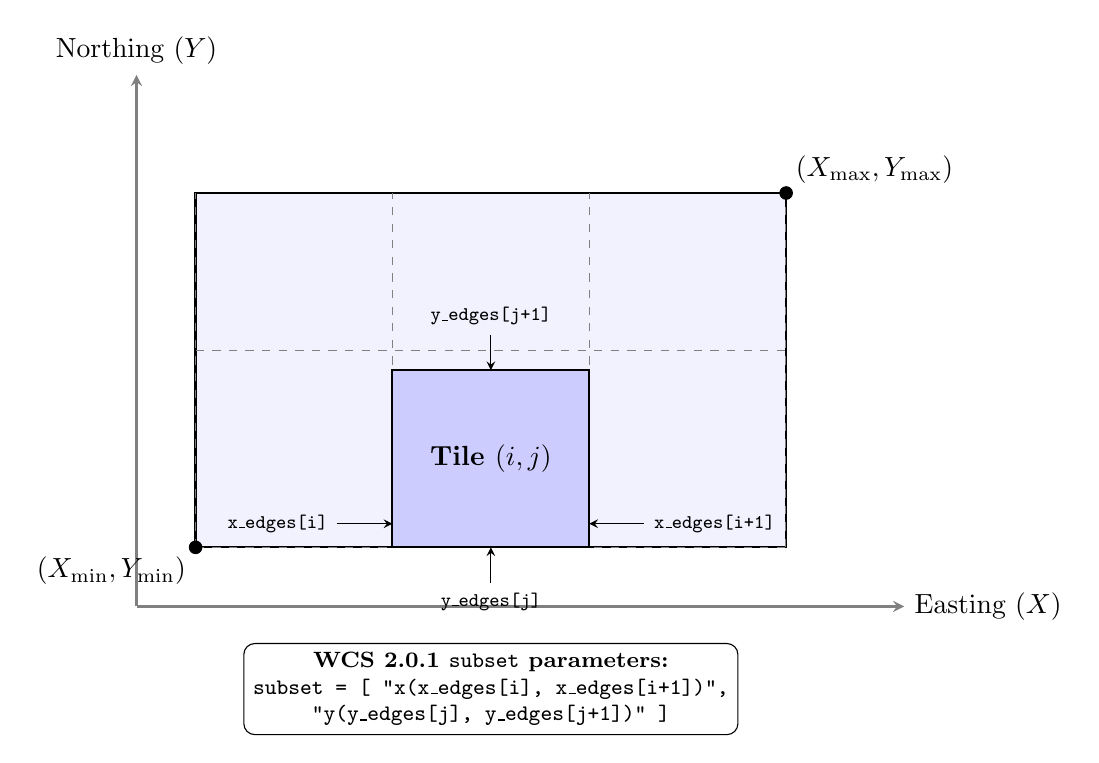
\begin{tikzpicture}[scale=1.5, >=stealth]
        % Draw axes
        \draw[->, thick, gray] (-0.5, -0.5) -- (6, -0.5) node[right, black] {Easting ($X$)};
        \draw[->, thick, gray] (-0.5, -0.5) -- (-0.5, 4) node[above, black] {Northing ($Y$)};

        % Draw the main bounding box (Global Study Area)
        \draw[thick, fill=blue!5] (0,0) rectangle (5,3);

        % Draw the grid (e.g., 3 columns, 2 rows)
        \draw[step=1.666cm, gray, dashed] (0,0) grid (5,3);

        % Highlight a specific tile (e.g., middle bottom: i=1, j=0)
        \draw[thick, fill=blue!20] (1.666, 0) rectangle (3.333, 1.5);

        % Label the highlighted tile
        \node at (2.5, 0.75) {\textbf{Tile $(i,j)$}};
        
        % Label local coordinates for the highlighted tile
        \draw[<-] (1.666, 0.2) -- (1.2, 0.2) node[left, font=\scriptsize] {\texttt{x\_edges[i]}};
        \draw[<-] (3.333, 0.2) -- (3.8, 0.2) node[right, font=\scriptsize] {\texttt{x\_edges[i+1]}};
        \draw[<-] (2.5, 0) -- (2.5, -0.3) node[below, font=\scriptsize] {\texttt{y\_edges[j]}};
        \draw[<-] (2.5, 1.5) -- (2.5, 1.8) node[above, font=\scriptsize] {\texttt{y\_edges[j+1]}};

        % Label global corners
        \filldraw[black] (0,0) circle (1.5pt) node[below left] {$(X_{\min}, Y_{\min})$};
        \filldraw[black] (5,3) circle (1.5pt) node[above right] {$(X_{\max}, Y_{\max})$};

        % Add descriptive callout for the WCS Request
        \node[align=center, font=\footnotesize, draw, fill=white, rounded corners] at (2.5, -1.2) {
            \textbf{WCS 2.0.1 \texttt{subset} parameters:}\\
            \texttt{subset = [ "x(x\_edges[i], x\_edges[i+1])",}\\
            \texttt{"y(y\_edges[j], y\_edges[j+1])" ]}
        };
    \end{tikzpicture}
    
    \caption[WCS 2.0.1 Spatial Tessellation Slicing]{Visual representation of the WCS spatial tessellation strategy. The global bounding 
    box computed in the target projection is partitioned into metric segments using the computed step limits. For each iteration, the 
    engine requests a precise sub-region (Tile $i,j$) mapped directly to the server's multi-dimensional slicing syntax.}
    \label{fig:wcs_tiling_strategy}
\end{figure}


\paragraph{D. In-Memory Mosaic Assembly and Standardized Persistence}

Once all individual sub-tiles are downloaded via HTTP as raw byte streams, the engine bypasses intermediate disk storage to optimize 
input/output bottlenecks. The byte streams are passed directly to an internal handling utility named \texttt{load\_raster\_from\_bytes}. 
This routine decodes the GeoTIFF streams and merges the individual spatial pieces into a unified, continuous mosaic array.

The compiled elevation array is forced into floating-point precision (\texttt{np.float32}), preserving the centimeter-level topography. 
Finally, this array is wrapped along with its geospatial metadata (Affine transform matrix, dimensions, and CRS) into a standardized 
\texttt{StaticRaster} object. This object acts as the formal, uniform interface utilized by all subsequent layers of the data pipeline, 
guaranteeing total structural compatibility when combining this terrestrial surface with marine datasets in the Topobathymetric Fusion 
Engine.


\subsubsection{Land Cover Generation Engine}

The Land Cover Generation Engine is a critical architectural component of the data pipeline, responsible for establishing the discrete 
physical and environmental features of the terrestrial surface. In a shallow water or cellular automata hydraulic simulation, boundary 
layer friction cannot be modeled as a uniform variable; instead, it depends directly on surface roughness. This engine, implemented via 
the \texttt{LandCoverGenerator} class, automates the ingestion, geometric filtering, and rasterization of high-resolution land use 
information. The resulting categorical matrix serves as the deterministic foundation for downstream parameterization of Manning's 
roughness coefficients ($n$).

\paragraph{A. Data Sourcing and WFS Feature Ingestion}

Unlike the terrain layers that fetch continuous numerical fields using the Web Coverage Service (WCS) protocol, the land cover engine 
relies on vector-based features. The system utilizes the Web Feature Service (WFS) provided by the Instituto Geográfico Nacional (IGN) 
to query the High-Resolution Land Cover System of Spain (SIOSE AR, updated to the 2020 dataset baseline). 

The connection routine handles spatial data extraction using a transactional request constrained by the study area's geographic limits. 
The \texttt{IgnClient} issues a spatial query filtering out features that intersect the configured bounding box. The server responds with 
rich vector geometries (polygons) paired with categorical attribute strings and classification taxonomy codes under the CC BY 4.0 
international license framework.

\paragraph{B. Spatial Context Inheritance and Exact Co-Registration}

To guarantee structural consistency within the simulator, all physical data layers must achieve absolute pixel-to-pixel alignment. Any 
spatial shift, offset, or discrepancy in resolution between the elevation surface and the friction layer would induce severe numerical 
instability in the hydraulic flux equations.

To eliminate this risk, the \texttt{LandCoverGenerator} enforces a strict execution dependency:

\begin{itemize}
    \item The pipeline interceptor verifies that the \texttt{topography} layer has been successfully compiled and resides in memory.
    \item The engine extracts the immutable \texttt{SpatialContext} of the topography layer, capturing its exact dimensions (width and 
    height), Coordinate Reference System (\texttt{target\_crs}), and the georeferencing Affine transformation matrix.
\end{itemize}

This inherited context is passed directly to the fetch routine, ensuring that the vector geometries are projected and bounded using the 
exact spatial blueprint of the terrain grid.

\paragraph{C. Vector-to-Raster Conversion Strategy}

Once the vector features are retrieved as a collection of shapes using the \texttt{fiona} library, they undergo an in-memory rasterization 
process. This step utilizes the advanced geometry parsing capabilities of \texttt{shapely} alongside the 
\texttt{rasterio.features.rasterize} compiler.

The engine iterates through the polygon collection, mapping each geographical shape to its respective integer taxid identifier according 
to the SIOSE/CODIIGE classification standard. Cells that do not intersect any explicit vector polygon are automatically assigned a 
standardized background nodata value. By utilizing direct matrix rasterization mapped against the pre-calculated Affine matrix, the 
pipeline completely avoids intermediate disk storage bottlenecks and eliminates spatial drift or interpolation artifacts.

\paragraph{D. Mathematical Mapping to Hydraulic Roughness (Manning's $n$)}

The final compiled raster stores discrete integer categories ($\mathbf{L}$). Within the hydraulic solver loop, this categorical matrix 
acts as the key for a deterministic Lookup Table (LUT) function. This mapping transforms a qualitative land class into a physical, 
quantitative friction coefficient.

Mathematically, the transformation function $f_{\text{rough}}$ maps each coordinate $(x,y)$ from the land cover domain to its corresponding 
Manning's roughness value ($n_M$):

\begin{equation}
    n_M(x,y) = f_{\text{rough}}\big(\mathbf{L}(x,y)\big)
\end{equation}

This parameterization ensures that when the shallow water equation solver computes the friction slope term ($S_f$), the momentum 
dissipation accurately reflects the sub-grid physical obstructions of the real-world territory. The resulting integer layer is safely 
encapsulated in a \texttt{StaticRaster} object with total structural metadata compliance.

\begin{figure}[htbp]
    \centering
    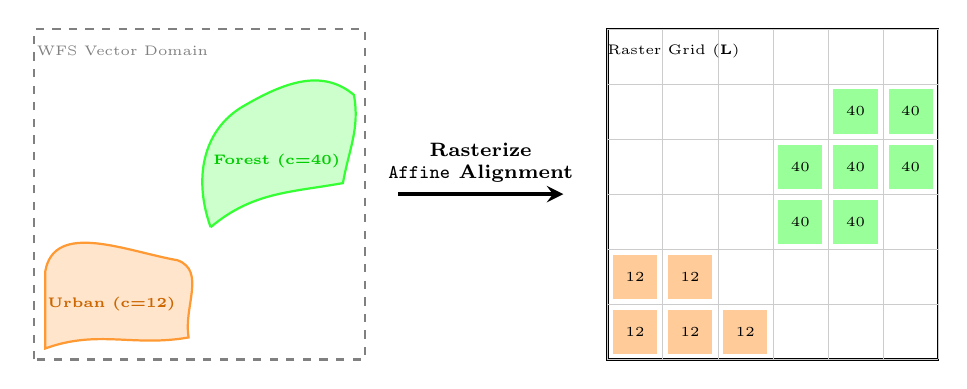
\begin{tikzpicture}[scale=1.4, >=stealth]
        % Left side: Vector Polygons (WFS)
        \draw[thick, gray, dashed] (0,0) rectangle (3,3);
        \node[font=\tiny, gray] at (0.8, 2.8) {WFS Vector Domain};
        
        % Arbitrary vector shapes
        \draw[fill=orange!20, draw=orange!80, thick] (0.1,0.1) to[out=20, in=190] (1.4,0.2) to[out=100, in=340] (1.3,0.9) to[out=170, in=80] (0.1,0.8) -- cycle;
        \node[font=\tiny\bfseries, color=orange!80!black] at (0.7,0.5) {Urban (c=12)};
        
        \draw[fill=green!20, draw=green!80, thick] (1.6,1.2) to[out=40, in=190] (2.8,1.6) to[out=80, in=280] (2.9,2.4) to[out=140, in=30] (1.9,2.3) to[out=210, in=110] cycle;
        \node[font=\tiny\bfseries, color=green!80!black] at (2.2,1.8) {Forest (c=40)};

        % Arrow with Rasterization label
        \draw[->, ultra thick, black] (3.3, 1.5) -- (4.8, 1.5) node[above, midway, font=\scriptsize\bfseries, align=center] {Rasterize\\ \texttt{Affine} Alignment};

        % Right side: Rasterized Grid
        \begin{scope}[shift={(5.2,0)}]
            \draw[thick, black] (0,0) rectangle (3,3);
            \draw[step=0.5cm, gray!40, ultra thin] (0,0) grid (3,3);
            \node[font=\tiny, black] at (0.6, 2.8) {Raster Grid ($\mathbf{L}$)};
            
            % Fill specific pixels to show rasterized representation
            \foreach \x/\y in {0/0, 0/1, 1/0, 1/1, 2/0} {
                \fill[orange!40] (\x*0.5+0.05, \y*0.5+0.05) rectangle (\x*0.5+0.45, \y*0.5+0.45);
                \node[font=\tiny] at (\x*0.5+0.25, \y*0.5+0.25) {12};
            }
            \foreach \x/\y in {3/2, 3/3, 4/2, 4/3, 5/3, 5/4, 4/4} {
                \fill[green!40] (\x*0.5+0.05, \y*0.5+0.05) rectangle (\x*0.5+0.45, \y*0.5+0.45);
                \node[font=\tiny] at (\x*0.5+0.25, \y*0.5+0.25) {40};
            }
        \end{scope}
    \end{tikzpicture}
    
    \caption[Vector-to-Raster Land Cover Conversion Mechanism]{Visual schematic of the vector-to-raster compilation. Irregular polygon 
    geometries downloaded via the IGN WFS protocol are mapped to discrete taxid integers and parsed into matrix cell coordinates using 
    the spatial context inherited from the topography layer.}
    \label{fig:vector_rasterization_mechanism}
\end{figure}


\subsubsection{Topobathymetric (Topo-Bathy) Fusion Engine}

The Topobathymetric (Topo-Bathy) Engine is a critical component of the data pipeline, responsible for generating a continuous, 
hydrologically sound elevation surface that bridges terrestrial topography with subaqueous bathymetry. In coastal or fluvial flood 
simulations, terrestrial digital elevation models frequently lack underwater morphologic data, treating water bodies as flat or 
zero-elevation surfaces. This engine, implemented via the \texttt{TopoBathyGenerator} class, resolves this limitation by dynamically 
fusing subaerial topography from the Instituto Geográfico Nacional (IGN) with marine bathymetry from the European Marine Observation and 
Data Network (EMODnet), guided by categorical land cover masks.

\paragraph{A. Multi-Source Ingestion and Layer Dependencies}

The execution of the Topo-Bathy engine follows a strict hierarchical dependency model within the simulation pipeline. Before the fusion 
can take place, the pipeline must successfully instantiate two antecedent layers:

\begin{itemize}
    \item \textbf{Topography Layer}: Provides the baseline Digital Elevation Model (MDT) fetched from the IGN WCS service, which defines 
    the target spatial context (bounding box, coordinate reference system, and spatial resolution).
    \item \textbf{Land Cover Layer}: Provides a rasterized categorical matrix based on the SIOSE/CODIIGE classification system fetched via 
    the IGN WFS service.
\end{itemize}

Once these dependencies are resolved, the engine invokes the \texttt{EmodnetClient} to fetch raw bathymetric data. The client automatically 
handles coordinate transformations, reprojecting the target bounding box into the native coordinate system of the EMODnet Web Coverage 
Service (\texttt{EPSG:4326}). It queries the \texttt{emodnet:mean} coverage layer, extracting raw numerical depths at the platform's native 
resolution of $0.00208333^{\circ}$ ($\approx 250\text{ meters}$) in high-bit-depth GeoTIFF format.

\paragraph{B. Spatial Co-Registration and Bilinear Resampling}

A major technical challenge is the structural discrepancy between the high-resolution topographic grid (typically defined in a metric 
projection such as ETRS89 / UTM Zone 30N, \texttt{EPSG:25830}) and the coarser, geographic grid of the EMODnet bathymetry array. 

To ensure exact grid cell alignment, the engine performs an in-memory spatial co-registration using the \texttt{rasterio.warp.reproject} 
framework. The raw bathymetric matrix is transformed to match the target shape, affine transformation matrix, and Coordinate Reference 
System (CRS) of the baseline topography. During this transformation, a \textbf{bilinear resampling} algorithm is applied. This 
interpolation method is mathematically essential to smooth out the transitions between the sparse bathymetric data points and the 
higher-resolution topographic grid, preventing artificial step-like artifacts along underwater slopes.

\paragraph{C. Categorical Masking and Topobathymetric Fusion}

The core contribution of this engine lies in its deterministic matrix fusion strategy. Instead of relying on a simple mathematical 
heuristic (such as taking the minimum or maximum value between layers, which introduces errors in low-lying coastal plains), the engine 
utilizes the categorical classification of the Land Cover layer as a spatial truth mask.

The algorithm defines a discrete set of hydrologically active water classes derived from the SIOSE/CODIIGE taxonomy:

\begin{equation}
    \mathcal{C}_{\text{water}} = \{47, 48, 49, 50, 51, 52, 53, 54\}
\end{equation}

Where these indices represent specific domains including salt marshes (47), rivers and water courses (50), reservoirs (52), and seas or 
oceans (54). 

During the fusion step, a boolean mask $\mathcal{M}$ is computed over the entire spatial domain, evaluating whether each individual pixel 
in the Land Cover matrix ($\mathbf{L}$) belongs to a water body:

\begin{equation}
    \mathcal{M}(x,y) = 
    \begin{cases} 
      1 & \text{if } \mathbf{L}(x,y) \in \mathcal{C}_{\text{water}} \\
      0 & \text{otherwise}
    \end{cases}
\end{equation}

Finally, the continuous topobathymetric elevation matrix ($\mathbf{E}_{\text{final}}$) is constructed by overwriting the baseline 
topography array ($\mathbf{T}$) with the reprojected bathymetric depths ($\mathbf{B}$) exclusively within the domain authorized by the 
mask $\mathcal{M}$:

\begin{equation}
    \mathbf{E}_{\text{final}}(x,y) = 
    \begin{cases} 
      \mathbf{B}(x,y) & \text{if } \mathcal{M}(x,y) = 1 \\
      \mathbf{T}(x,y) & \text{if } \mathcal{M}(x,y) = 0
    \end{cases}
\end{equation}

This procedure ensures that terrestrial landmarks, urban expansion zones, and agricultural fields remain perfectly untouched, while 
riverbeds and maritime basins are injected with accurate depth metrics.

\paragraph{D. Standardized Persistence and Continuous Surface Outputs}

The final step wraps the unified matrix into a structured \texttt{StaticRaster} metadata instance, inheriting the exact affine parameters 
and spatial properties of the baseline topography to guarantee total compatibility with subsequent steps of the flooding pipeline (such 
as roughness map generation or shallow water equation solver initializations).

The dataset retains full floating-point precision (\texttt{np.float32}) throughout the execution loop. When saved to disk under the 
configuration framework, it preserves detailed topographic integrity, ensuring that the critical interface between land and sea is 
represented as a smooth, physically accurate, and continuous mathematical surface.


\subsubsection{Initial Water Depth Estimation Engine}

The Initial Water Depth Engine is responsible for establishing the initial hydraulic state ($t=0$) of the simulation environment. In 
shallow water equations and hydraulic cellular automata, the state of the global domain is evaluated using conserved variables, where 
water depth constitutes the primary scalar field. This engine, implemented via the \texttt{WaterDepthGenerator} class, determines the 
spatial distribution and volume of standing water bodies across riverbeds, reservoirs, and coastal basins prior to the first computational 
time step, eliminating the need for manual, error-prone boundary initialization.

\paragraph{A. Pipeline Dependencies and Synchronous Ingestion}

The extraction of the initial water column follows an algebraic post-processing model that requires the strict pre-execution of two 
antecedent baseline layers. The pipeline orchestration framework blocks the execution of the \texttt{WaterDepthGenerator} until the 
following matrices are compiled and held in memory:

\begin{itemize}
    \item \textbf{Topography Layer ($\mathbf{T}$)}: Represents the raw terrestrial surface model derived from the IGN WCS endpoint. 
    Crucially, over active water bodies, satellite or airborne radar sensors often register the upper water surface or a flat reflected 
    pane rather than the underlying channel bed.
    \item \textbf{Topobathymetry Layer ($\mathbf{E}_{\text{final}}$)}: Represents the continuous fused elevation model, where subaqueous 
    regions have been actively injected with EMODnet depth data, effectively carving out the true bathymetric profile of the basins.
\end{itemize}

Once both layers are validated, the engine inherits the immutable \texttt{SpatialContext} from the baseline topography layer to ensure 
perfect cell alignment and grid size uniformity.

\paragraph{B. Algebraic Extraction of the Water Column}

The fundamental operating principle of this engine is the mathematical extraction of the fluid column thickness by computing the vertical 
difference between the superficial topography and the subaqueous bed. 

Mathematically, for each discrete coordinate $(x,y)$ in the simulation grid, the raw water depth $\mathbf{W}_{\text{raw}}(x,y)$ is 
calculated by subtracting the fused topobathymetric matrix from the baseline surface topography array:

\begin{equation}
    \mathbf{W}_{\text{raw}}(x,y) = \mathbf{T}(x,y) - \mathbf{E}_{\text{final}}(x,y)
\end{equation}

Where:
\begin{itemize}
    \item Over terrestrial land covers (e.g., urban or agricultural zones), both layers contain identical values 
    ($\mathbf{T}(x,y) = \mathbf{E}_{\text{final}}(x,y)$), resulting in a raw value of zero.

    \item Over valid water bodies, the topobathymetric surface dips significantly lower than the superficial topography 
    ($\mathbf{E}_{\text{final}}(x,y) < \mathbf{T}(x,y)$), yielding a positive value that represents the exact physical thickness of the initial standing water column.
\end{itemize}

\paragraph{C. Numerical Firewall and Noise Filtering}

In real-world geomorphological data pipelines, combining multi-source datasets frequently introduces vertical datum discrepancies, 
satellite sensor noise, or minor horizontal co-registration shifts along steep river banks. If left uncorrected, these geometric errors 
would yield negative values during the matrix subtraction ($\mathbf{T}(x,y) < \mathbf{E}_{\text{final}}(x,y)$). In a hydraulic solver, a 
negative fluid depth is a catastrophic mathematical anomaly that triggers immediate numerical divergence in the flux calculus.

To prevent this, the engine implements a non-linear numerical firewall using an element-wise maximum clipping function via 
\texttt{np.maximum}:

\begin{equation}
    \mathbf{W}_{\text{clean}}(x,y) = \max\big(0.0, \, \mathbf{W}_{\text{raw}}(x,y)\big)
\end{equation}

This operation ensures that any sub-grid pixel noise or vertical misalignment over solid ground is safely clamped to a physically 
consistent value of exactly $0.0\text{ meters}$, protecting the downstream stability of the cellular automata state tensor.

\begin{figure}[htbp]
    \centering
    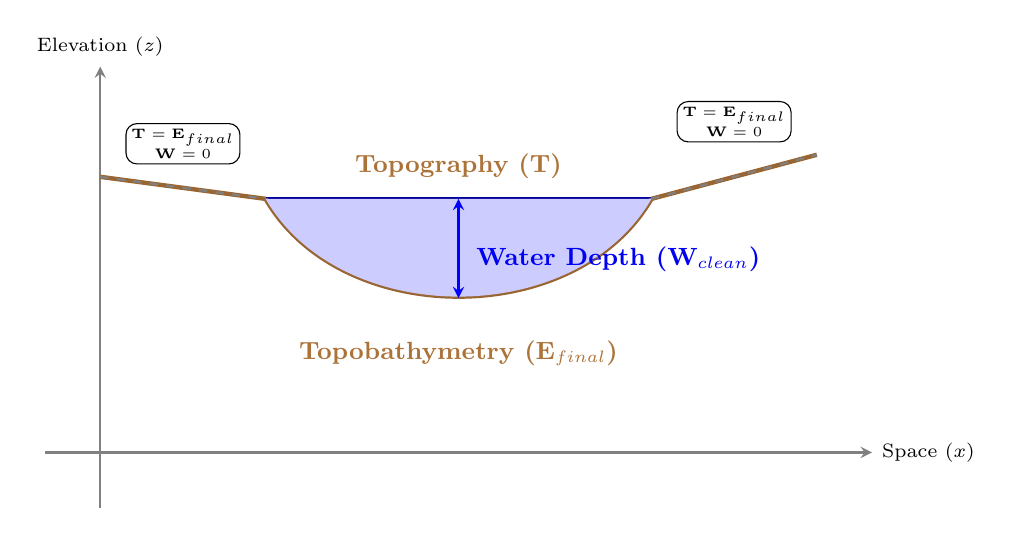
\begin{tikzpicture}[scale=1.4, >=stealth]
        % Draw Coordinates
        \draw[->, thick, gray] (0,-1) -- (0,3) node[above, black, font=\scriptsize] {Elevation ($z$)};
        \draw[->, thick, gray] (-0.5,-0.5) -- (7,-0.5) node[right, black, font=\scriptsize] {Space ($x$)};
        
        % Left Bank (Terrestrial)
        \draw[ultra thick, brown!80!black] (0,2) -- (1.5,1.8);
        \draw[thick, dashed, gray] (0,2) -- (1.5,1.8);
        
        % River Section - Topography Layer T (Flat water surface line)
        \draw[ultra thick, blue!60!black] (1.5,1.8) -- (5,1.8);
        
        % River Section - Topobathymetry Layer E_final (Carved bed profile)
        \draw[ultra thick, brown!80!black] (1.5,1.8) to[out=-60, in=240] (5,1.8);
        
        % Right Bank (Terrestrial)
        \draw[ultra thick, brown!80!black] (5,1.8) -- (6.5,2.2);
        \draw[thick, dashed, gray] (5,1.8) -- (6.5,2.2);
        
        % Shading the initial water depth area
        \path[fill=blue!20] (1.5,1.8) to[out=-60, in=240] (5,1.8) -- cycle;
        
        % Labels
        \node[font=\small\bfseries, color=brown!90!black] at (3.25, 2.1) {Topography ($\mathbf{T}$)};
        \node[font=\small\bfseries, color=brown!90!black] at (3.25, 0.4) {Topobathymetry ($\mathbf{E}_{\text{final}}$)};
        \node[font=\small\bfseries, color=blue!95!black] at (4.7, 1.25) {Water Depth ($\mathbf{W}_{\text{clean}}$)};
        
        % Inundation arrows
        \draw[<->, thick, blue] (3.25, 1.8) -- (3.25, 0.9);
        
        % Terrestrial label showing T = E_final
        \node[font=\tiny, align=center, fill=white, inner sep=2pt, draw, rounded corners] at (0.75, 2.3) {$\mathbf{T} = \mathbf{E}_{\text{final}}$\\$\mathbf{W} = 0$};
        \node[font=\tiny, align=center, fill=white, inner sep=2pt, draw, rounded corners] at (5.75, 2.5) {$\mathbf{T} = \mathbf{E}_{\text{final}}$\\$\mathbf{W} = 0$};
    \end{tikzpicture}
    
    \caption[Initial Water Depth Extraction Mechanism]{Cross-sectional profile illustrating the mathematical extraction of the initial 
    water column. Over solid terrain, the topography and topobathymetry profiles are identical, yielding a depth of zero. Over water 
    courses, the difference between the flat surface captured by $\mathbf{T}$ and the channel bed carved by $\mathbf{E}_{\text{final}}$ 
    defines the fluid depth tensor.}
    \label{fig:water_depth_mechanism}
\end{figure}

\paragraph{D. Serialization and Pipeline State Encapsulation}

The resulting filtered matrix is encapsulated within a standard \texttt{StaticRaster} data model, carrying forward the spatial metadata 
references inherited from the upstream nodes. 

By maintaining total structural compatibility and strict floating-point precision (\texttt{np.float32}), this layer provides the cellular 
automata engine with a deterministic map of standing water columns. This map defines the boundary flux potentials and hydrostatic pressures 
at $t=0$, enabling a physically accurate and clean initialization of the dynamic routing equations.


\subsubsection{Rainfall Intensity Engine}

The Rainfall Intensity Engine is a critical component of the data pipeline, responsible for transforming discrete, 
asynchronous meteorological observations into a continuous spatiotemporal 3D tensor ($Time \times Y \times X$). 
This engine ensures that the flood simulator receives high-resolution precipitation forcing data, accounting for both 
the temporal evolution of storms and the geographic variations influenced by terrain.

The engine is architected following a modular approach, separating the concerns of data acquisition, spatial 
interpolation, and temporal management.


\paragraph{A. System Architecture and Orchestration}

The orchestration of the rainfall data flow is managed by the RainfallGenerator class. This component acts as the 
high-level controller that integrates three distinct sub-systems:

\begin{enumerate}
    \item \textbf{Extraction Layer (RainDataManager)}: Coordinates multiple data sources (e.g., SAIH Júcar) to fetch 
    raw precipitation records.
    \item \textbf{Interpolation Layer (KrigingInterpolator)}: Applies advanced geostatistical methods to generalize 
    point data into a continuous surface.
    \item \textbf{Integration Layer}: Conforms the resulting grids into the simulation's global grid structure, ensuring 
    CRS (Coordinate Reference System) consistency and temporal alignment.
\end{enumerate}

\begin{figure}[htbp]
    \centering
    
\includegraphics[width=1.0\textwidth]{chapter_4/rainfall_architecture.pdf}
    
    \caption[UML Class Diagram of the RainfallGenerator system architecture]{UML Class Diagram of the 
    \texttt{RainfallGenerator} system architecture. The diagram depicts the structural composition of the module, 
    highlighting the Separation of Concerns (SoC) across the Extraction, Interpolation, and Integration layers. 
    Directional dashed arrows illustrate the flow of specific data structures (\texttt{StationRainData}, 
    \texttt{RainDataPoint}) as they are fetched from external sources and processed into a unified spatial grid.}
    \label{fig:rainfall_architecture}
\end{figure}


\paragraph{B. Multi-Source Data Acquisition}

To ensure reliability and coverage, the engine employs a facade pattern through the RainDataManager. This allows the 
system to aggregate data from various meteorological networks simultaneously.

\begin{itemize}
    \item \textbf{Standardized Fetching Interface}: All data sources implement a BaseFetcher interface, which enforces 
    methods for station discovery, spatial filtering (within the simulation bounding box), and reprojection of 
    coordinates to the target EPSG.
    \item \textbf{SAIH Júcar Integration}: A specialized fetcher (\texttt{SAIHJucarFetcher}) is implemented to scrape historical 
    data from the "Confederación Hidrográfica del Júcar". This involves a complex process of parsing HTML for station 
    metadata and extracting precipitation values from PDF reports using specialized parsing libraries.
    \item \textbf{Data Normalization}: Raw measurements, often provided in heterogeneous formats or accumulation periods, 
    are normalized into RainDataPoint objects, representing intensity in mm/h at specific spatial coordinates.
\end{itemize}

\begin{figure}[htbp]
    \centering
    
\includegraphics[width=0.85\textwidth]{chapter_4/rainfall_extraction_sequence.pdf}
    \caption[Sequence diagram illustrating the multi-source data acquisition workflow]{The process highlights the 
    role of the \texttt{SAIHJucarFetcher} in station discovery, spatial bounding box filtering, coordinate reprojection, 
    and the subsequent extraction and normalization of precipitation data from PDF reports.}
    \label{fig:rainfall_extraction_sequence}
\end{figure}


\paragraph{C. Spatial Interpolation: Kriging with External Drift (KED)}

The engine implements Kriging with External Drift (KED) via the KrigingInterpolator class. Standard interpolation methods 
(like IDW or Nearest Neighbor) often fail to capture the orographic effect—the phenomenon where higher elevations 
typically experience higher precipitation intensities. By using a Digital Elevation Model (DEM) as a secondary variable 
(drift), the engine produces meteorologically consistent surfaces.

The interpolation process follows a rigorous five-step geostatistical workflow:

\begin{itemize}
    \item \textbf{Drift Estimation}: The system extracts elevation values from the DEM at each meteorological station's 
    coordinates. It then fits a linear regression model to establish the relationship:

    $$P_{trend} = \alpha + \beta \cdot Z$$

    where $P_{trend}$ is the predicted precipitation and $Z$ is the elevation.

    \item \textbf{Residual Calculation}: To isolate the spatial autocorrelation, the engine subtracts the elevation trend 
    from the observed values at the stations:

    $$R(s_i) = P(s_i) - (\alpha + \beta \cdot Z(s_i))$$

    \item \textbf{Variogram Modeling}: Using the gstools library, the engine calculates the experimental variogram of the 
    residuals. It automatically fits a theoretical model (e.g., Spherical, Gaussian, or Exponential) to define the spatial 
    structure, determining parameters such as the nugget, sill, and range.
    \item \textbf{Ordinary Kriging of Residuals}: The engine performs Ordinary Kriging on the residuals across the entire 
    grid. This ensures that local deviations from the elevation trend are smoothly honors at the station locations.
    \item \textbf{Final Reconstruction}: The linear trend is reapplied to the kriged residual surface for every pixel in 
    the grid:

    $$P_{final}(x, y) = R_{krige}(x, y) + (\alpha + \beta \cdot Z(x, y))$$
\end{itemize}

\begin{figure}[htbp]
    \centering
    
\includegraphics[width=0.8\textwidth]{chapter_4/ked_algorithm_flow.pdf}
    
    \caption[Flowchart of the Kriging with External Drift (KED) algorithm]{Flowchart of the Kriging with External 
    Drift (KED) algorithm. The diagram illustrates the branching process where the global orographic trend is 
    calculated across the entire DEM grid concurrently with the geostatistical interpolation (Ordinary Kriging) of 
    the local residuals. Both branches converge in the final reconstruction step to produce the meteorologically 
    consistent rainfall surface.}
    \label{fig:ked_algorithm_flow}
\end{figure}


\paragraph{D. Temporal Management and Tensor Assembly}

The RainfallGenerator transforms the sequence of interpolated 2D grids into a structured 3D temporal tensor.

\begin{itemize}
    \item \textbf{Temporal Resampling}: Since station observations and simulation time steps may not align, the engine 
    performs temporal filtering. For each simulation frame, it identifies "active" data points whose measurement windows 
    cover the current timestamp.
    \item \textbf{Resolution Downsampling}: To optimize performance, the engine includes a \_downsample\_dem utility. This 
    allows the Kriging process to run on a coarser version of the DEM if requested, significantly reducing the computational 
    cost of the variogram fitting without losing the general topographic influence.
    \item \textbf{Data Integrity}: The engine handles edge cases, such as periods with insufficient active stations, by 
    defaulting to zero-rainfall grids or logging warnings to prevent the simulation from receiving uninitialized memory.
\end{itemize}

\begin{figure}[htbp]
    \centering
    
\includegraphics[width=0.7\textwidth]{chapter_4/rainfall_tensor_assembly.pdf} 
    \caption[3D spatiotemporal rainfall tensor assembly]{Conceptual representation of the 3D spatiotemporal data 
    cube (\texttt{DynamicRaster}). Each 2D spatial mesh represents an interpolated rainfall grid at a specific time 
    step ($\Delta t$). The chronological stacking illustrates the temporal filtering process, which maintains data 
    integrity by inserting zero-rainfall grids when no active measurement windows are available. Spatial resolution 
    can be optionally optimized via the \texttt{\_downsample\_dem} utility prior to tensor assembly.}
    \label{fig:rainfall_tensor_assembly}
\end{figure}


\subsection{Pipeline Execution and Computational Optimizations}

The conceptual GIS-to-tensor pipeline and the subsequent simulation engine were implemented focusing on computational efficiency, memory 
alignment, and the mitigation of processing overheads inherent to large-scale geospatial datasets.

\paragraph{A. Automated Data Ingestion and ETL Processing}

The ingestion of heterogeneous raw data formats—including legacy and specialized formats such as HIF and IDRISI—is managed via the 
Geospatial Abstraction Layer (GDAL). The developed ETL script utilizes this library to programmatically parse spatial metadata, automate 
the transformation of geographic coordinates to the target UTM 30N projection, and execute the grid resampling routines described in the 
methodology.

\paragraph{B. Vectorized Simulation Engine and Hardware Acceleration}

To execute the cellular automata simulation efficiently, the tensorized data structure $(C, H, W)$ is mapped directly onto contiguous 
memory blocks. Rather than relying on traditional, computationally expensive cell-by-cell loops to evaluate transition rules, the 
simulation engine is built entirely on vectorized execution.Transition rules are translated into element-wise matrix operations and 
array shifts. This design choice completely bypasses high-level interpreter loop overheads, allowing the underlying hardware to leverage 
Single Instruction, Multiple Data (SIMD) architectures. Consequently, spatial state updates across the entire $H \times W$ grid are 
processed in parallel at the hardware level, significantly reducing execution time for high-resolution river basin simulations.


\subsection{System Observability: Multi-Sink Logging Architecture}
\label{subsec:logging_subsystem}

Long-running environmental simulations demand rigorous system observability to monitor operational health and ensure mathematical 
reproducibility. To satisfy this requirement, the pipeline implements an asynchronous Multi-Sink Logging Pattern initialized at the 
application entry point (\texttt{main.py}). This architecture completely decouples high-level telemetry generation from persistent disk 
logging, optimization-driven filtering, and execution auditing.

\subsubsection{Dual-Sink Stratification and Thresholding}

To manage the massive volume of diagnostic data generated during large-scale raster transformations, the subsystem splits telemetry into 
two distinct streams based on severity thresholds:

\begin{itemize}
    \item \textbf{Transient Console Sink (Standard Output)}: Operating under an \texttt{INFO} severity threshold, this sink provides 
    immediate, human-readable feedback without cluttering the terminal interface. It utilizes localized, color-coded markup tags (e.g., 
    \texttt{<green>SUCCESS</green>}) to highlight macro-level milestones, focusing exclusively on system initialization parameters, the 
    resolved topological execution order of the layers, and final generation states.

    \item \textbf{Persistent File-Based Ledger (\texttt{log.txt})}: Configured with an exhaustive \texttt{TRACE} severity threshold, this 
    disk-bound sink captures a granular technical history for post-execution audits. It records explicit spatial file paths, sub-pixel 
    interpolation warnings, the precise affine transformation matrices extracted during \textsl{Rasterio} geospatial compliance loops, and 
    the exact physical memory addresses of the newly instantiated tensors.
\end{itemize}

\begin{figure}[htbp]
    \centering
    
\includegraphics[width=0.7\textwidth]{chapter_4/logging_architecture}
    \caption{Logging Subsystem Architecture and Multi-Sink Flow}
    \label{fig:logging_architecture}
\end{figure}

\subsubsection{Runtime Traceability and Cross-Language Error Handling}

To operate effectively within a complex, hybrid software environment, the logging engine enriches intercepted events with critical runtime 
metadata. Each log entry incorporates automated contextual breadcrumbs utilizing a \texttt{\{name\}:\{line\}} format string, instantly 
pinpointing the specific script and line number where an anomaly or spatial misalignment occurs.

Furthermore, the data pipeline implements structured exception backtracing via automated context managers (\texttt{logger.exception()}) 
inside its primary execution loops. In the event of a runtime failure, the system captures, formats, and materializes the complete execution 
stack trace. This capability is paramount for diagnosing low-level, C++-linked memory or numerical exceptions propagated back through 
foreign function interfaces, which would otherwise be obfuscated or lost within standard high-level interpreter tracebacks.

\subsubsection{Asynchronous Performance and Retention Policies}

To guarantee that high-frequency disk writing does not introduce critical I/O bottlenecks during intensive tensorization, the persistent 
file sink relies entirely on non-blocking, asynchronous execution loops. Storage footprints are controlled deterministically through a 
strict rotation and retention policy: the active log file is automatically rotated upon reaching a 10~MB threshold and immediately 
compressed into a ZIP archive, safeguarding system resources during multi-scenario computational campaigns.


\subsection{Pipeline Execution Artifacts and Output Layout}
\label{subsec:execution_results}

Upon a successful lifecycle completion, the data pipeline outputs a strictly structured, deterministic directory tree. This standardized 
filesystem layout establishes the absolute data contract required by the downstream, high-performance C++ simulation core, which expects 
physical environmental parameters at immutable relative boundaries.

The root of the execution workspace is dynamically named utilizing an execution timestamp (\texttt{output\_simulation\_YYYYMMDD/}) to 
isolate distinct simulation scenarios. Within this root, the orchestrator segregates transient logs, static geographic boundaries, and 
time-varying spatial tensor cubes into specialized sub-directories, as detailed in Figure~\ref{fig:data_pipeline_output_structure}.

\begin{figure}[htbp]
    \centering
    \footnotesize
    \begin{forest}
      for tree={
        folder,   
        font=\ttfamily,
        grow'=0,
      }
    [output\_simulation\_YYYYMMDD/
      [logs/
        [\filedesc{log.txt}{Full execution tracing ledger}]
      ]
      [elevation/
        [\filedesc{elevation.doc}{Base terrain geometry (IDRISI)}]
        [\file{elevation.img}]
        [visualization/
          [elevation.png]
        ]
      ]
      [roughness/
        [\filedesc{roughness.doc}{Manning's n descriptor (IDRISI)}]
        [\file{roughness.img}]
        [visualization/
          [roughness.png]
        ]
      ]
      [rainfall/
        [\filedesc{rainfall.hif}{3D Spatiotemporal Rainfall Cube descriptor}]
        [\file{attrs.json}]
        [\file{000000.img}]
        [\file{000001.img}]
        [\file{...}]
        [visualization/
          [\filedesc{rainfall\_frame\_001.png}{Temporal snapshots for diagnostic verification}]
          [\file{...}]
        ]
      ]
      [water\_depth/
        [\filedesc{water\_depth.doc}{Initial hydraulic boundary state (IDRISI)}]
        [\file{water\_depth.img}]
        [visualization/
          [water\_depth.png]
        ]
      ]
    ]
    \end{forest}
    \caption[Standardized Pipeline Output Directory Structure]{Standardized hierarchical directory structure generated by the data pipeline for downstream C++ core consumption.}
    \label{fig:data_pipeline_output_structure}
\end{figure}

Each subdirectory is configured with an automated diagnostics engine that generates a parallel \texttt{visualization/} folder. This folder 
isolates standard graphic formats (e.g., \texttt{.png} spatial grids) generated post-processing, allowing researchers to perform instant 
visual verification of the alignment, boundaries, and spatial integrity of the input datasets prior to triggering the main numerical engine.
